% REMEMBER: You must not plagiarise anything in your report. Be extremely careful.

\documentclass{l4proj}


%
% put any additional packages here
%
\usepackage{forest}

\begin{document}

%==============================================================================
%% METADATA
\title{Carbon Emissions Estimation in Edge Cloud Computing Simulations}
\author{James A. Nurdin}
\date{September 19, 2023}

\maketitle

%==============================================================================
%% ABSTRACT
\begin{abstract}
    \vskip 0.5em
    With the ever-increasing energy requirements from cloud computing, the fog computing paradigm was introduced to distribute workload away from large-scale data centres by processing information at the network's edges.
    Recently, many energy-aware fog computing simulators have been introduced to model the power consumption of these fog computing networks.
    However, most overlook how this energy is provided to the network and the greenhouse gasses released in doing so.
    As the ICT industry continues to increase its carbon emissions, it is crucial that we consider the impact fog computing has on the environment.

    We propose ECO-LEAF, an energy-aware fog computing simulator capable of supplying this energy demand to network infrastructure,
    By considering the availability of power sources, ECO-LEAF is able to model how power is distributed across network infrastructure and provide estimations of their carbon emissions as a consequence of consuming this energy.
    ECO-LEAF achieves this by utilising historical datasets to provide accurate and precise information on how energy availability and environmental impact fluctuate over time and location.

    To evaluate the effectiveness of this model, we produced scenarios in a precision agriculture setting. This provided a practical context to showcase the tool's research and industrial capabilities.
    By referencing goals for ECO-LEAF, the scenarios were used to identify that ECO-LEAF achieved the ability to model power sources in fog networks and could determine how power was efficiently distributed across the infrastructure.

        \textbf{Index Terms — Simulation, Modeling, Fog Computing, Energy Consumption, Power Sources, Carbon Intensity, Power Availability}
\end{abstract}

%==============================================================================

% EDUCATION REUSE CONSENT FORM
% If you consent to your project being shown to future students for educational purposes
% then insert your name and the date below to  sign the education use form that appears in the front of the document. 
% You must explicitly give consent if you wish to do so.
% If you sign, your project may be included in the Hall of Fame if it scores particularly highly.
%

%
\def\consentname {James Andrew Nurdin} % your full name
\def\consentdate {7 March 2024} % the date you agree
%
\educationalconsent
%==============================================================================
\tableofcontents
%==============================================================================
%% Notes on formatting
%==============================================================================
% The first page, abstract and table of contents are numbered using Roman numerals and are not
% included in the page count. 
%
% From now on pages are numbered
% using Arabic numerals. Therefore, immediately after the first call to \chapter we need the call
% \pagenumbering{arabic} and this should be called once only in the document. 
%
% Do not alter the bibliography style.
%
% The first Chapter should then be on page 1. You are allowed 40 pages for a 40 credit project and 30 pages for a 
% 20 credit report. This includes everything numbered in Arabic numerals (excluding front matter) up
% to but excluding the appendices and bibliography.
%
% You must not alter text size (it is currently 10pt) or alter margins or spacing.
%
%
%==================================================================================================================================
%
% IMPORTANT
% The chapter headings here are **suggestions**. You don't have to follow this model if
% it doesn't fit your project. Every project should have an introduction and conclusion,
% however. 
%
%==================================================================================================================================
\chapter{Introduction}\label{chp:intro}

% reset page numbering. Don't remove this!
\pagenumbering{arabic} 


%Why should the reader care about what are you doing and what are you actually doing?
%\section{Guidance}

%\textbf{Motivate} first, then state the general problem clearly.

%This is the key question for any writing. Your reader:
%    is a trained computer scientist: \emph{don't explain basics}.
%    has limited time: \emph{keep on topic}.
%    has no idea why anyone would want to do this: \emph{motivate clearly}
%    might not know \emph{anything} about your project in particular:
%    \emph{explain your project}.
%    but might know precise details and check them: \emph{be precise and
%    strive for accuracy.}
%    doesn't know or care about you: \emph{personal discussions are irrelevant}.

%- motivation:
%    - i'm missing energy sources, including multiple sources, with both grid and on-site renewables, and how these have different carbon intensities (at different times and different locations)
%    - i'm also missing a bit more of a problem: this is already quite focused on abilities and framework features

\section{Motivation}\label{intro:subsec:motivation}
\citep{en12010184}
Over the past decade, the information and communication technology (ICT) industry has drastically increased its share of global energy consumption and, consequently, its emission of greenhouse gasses.
A recent study approximates that the ICT industry emits around 2.1-3.9 \% of global greenhouse gas emissions \citep{current_energy_consumption}.
With the ever-increasing energy requirements from power-intensive services like cloud computing, the ICT industry is expected to consume even more of global greenhouse gas emissions in the future \citep{co2Challenges}.
Consequently, as the industry continues to demand larger energy requirements, it imposes a more significant environmental threat to meet this demand.
In an attempt to circumvent this, the discipline of sustainable computing has become a vital area of study within computer science to reduce the industry's impact on the environment.

One proposed solution currently in efforts to help decentralise this energy demand is a distributed computation platform called edge/fog computing.
Rather than carrying out centralised processing at the centre of a network, the technique sees to locally execute processes at the edge on less power-intensive devices before being transported to the intended destination.
To facilitate research and industrial applications of the platform, various software tools currently exist to model these particular environments by considering interactions of network infrastructure and the running of applications inside a simulation space.
In order to effectively model their environments, many tools take into account a range of considerations that are unique to edge/fog computing.
These considerations might reflect the granularity and reliability of communications within the network \citep{FogNetSim}, the representation of network infrastructure \citep{ENIGMA}, and even the optimisation of a network's performance \citep{EdgeCloudSim}.
However, only a few available tools currently emphasise how power consumption can be modelled.
One such tool, LEAF (Large Energy-Aware Fog computing environments) \citep{leaf2021}, was previously developed to provide analytical power modelling inside an edge/fog computing simulation.

Despite the variety of edge/fog computing simulation tools that incorporate power modelling into their environments, many of these tools have yet to model how power can be provided to network infrastructure and estimate the carbon footprint produced as a result.
The proposed solution, Energy sources And Carbon emission Offerings in Large Energy-Aware Fog computing environments (ECO-LEAF), seeks to introduce the ability to model various battery, grid, and on-site renewable power sources to provide energy to network infrastructure.
In particular, ECO-LEAF also aims to consider how these power sources can vary in energy availability and carbon intensity at various times and locations.
Finally, using these models, ECO-LEAF aims to estimate carbon footprints for infrastructure within the network.
By introducing these tools, ECO-LEAF aims to provide further research and industrial opportunities to utilise fog computing by being able to take into consideration the carbon produced as a result of running the environment.

%   - estimation of carbon emissions is one aim, but being able to assess "how exploiting opportunities can reduce the carbon footprint" is another, yet that isn't presented in much detail
%    - "demonstrate the accuracy of estimated carbon footprints of smaller scenarios": that's interesting. how will you demonstrate the accuracy?

\section{Goals}\label{intro:subsec:goals}
\textbf{\textit{(1) Introduce a means of modelling power sources}}
(1.1)\label{goal1.1} The first main goal ECO-LEAF should consider is the heterogeneity of real power sources and allow for the modelling of any kind of power source inside the environment, such as grid, solar, or even battery power.
(1.2)\label{goal1.2} Users should be able to express precisely what type of power sources they want by defining their own or configuring those provided by ECO-LEAF.
This is important because the unique properties of a power source can provide different values for a given simulation.
(1.3)\label{goal1.3} In addition to this, power sources should be able to fluctuate in their power availability (PA) as a consequence of environmental conditions.
(1.4)\label{goal1.4} Because of this, power sources should only also be able to distribute the power they can provide.
(1.5)\label{goal1.5} Finally, ECO-LEAF should also be able to determine how power from these various sources is distributed amongst devices in the environment.

\textbf{\textit{(2) Provide carbon footprints for consuming power}}
(2.1)\label{goal2.1} The second main goal in extending LEAF is to provide estimations of carbon footprints from entities within the simulation.
(2.2)\label{goal2.2} Therefore, ECO-LEAF should provide a direct means to translate energy consumed into greenhouse gas emissions.
(2.3)\label{goal2.3} The user should also be able to define how applications are placed on the infrastructure by considering power sources.
(2.4)\label{goal2.4} Finally, the simulation should also model how the quantity of greenhouse gas emissions can vary due to conditions in the environment.

\textbf{\textit{(3) Capturing and displaying results}}
Another goal for ECO-LEAF is to provide the user with a means to capture and display simulation results.
(3.1)\label{goal3.1} First, ECO-LEAF should keep track of values that describe the state of the environment at any given moment during the simulation.
(3.2)\label{goal3.2} The user should be able to probe the model afterwards and retrieve information concerning carbon emissions and power measurements from devices and power sources.
(3.3)\label{goal3.3} The user should also be able to request that data about the simulation be saved to a file and stored in a convenient structure for later use.
This is particularly important because the simulation models many aspects of the environment and will handle large amounts of data.

\textbf{\textit{(4) Introduce example scenarios}}
The last goal for ECO-LEAF is to see that during the development of the framework, a series of examples are produced to demonstrate the capabilities of the new features.
These examples would ensure the feature's usability during development and demonstrate its purpose to new users wishing to use ECO-LEAF.
By gradually introducing new features, the main focus of an example can be on demonstrating their functionality.

\section{Dissertation Outline}
The structure of the dissertation consists of eight chapters, which are outlined as follows:
\begin{itemize}
    \item \textbf{Chapter 2} presents general concepts discussed frequently throughout the dissertation to provide further context to ECO-LEAF.
    \item \textbf{Chapter 3} explores related works of ECO-LEAF by discussing the surrounding models and tools in edge/fog computing.
    \item \textbf{Chapter 4} identifies the expectations of ECO-LEAF and provides a detailed list of requirements that the product should have.
    \item \textbf{Chapter 5} discusses the design behind the proposed solution by covering an abstract overview of the core principles behind ECO-LEAF.
    \item \textbf{Chapter 6} explains how these concepts were realised and able to introduce power sources and carbon footprints in the ECO-LEAF framework.
    \item \textbf{Chapter 7} introduces the evaluation strategy and demonstrates ECO-LEAF's functionality through a series of scenarios, identifying how the previous goals defined were met.
    \item Finally, \textbf{Chapter 8} concludes the dissertation with a summary of the project, limitations of ECO-LEAF, and future work for the framework.
\end{itemize}
%\subsection{References and style guides}
%There are many style guides on good English writing. You don't need to
%read these, but they will improve how you write.
%    \emph{How to write a great research paper}~\cite{Pey17} (\textbf{recommended}, even though you aren't writing a research paper)
%    \emph{How to Write with Style} \cite{Von80}. Short and easy to read. Available online.
%    \emph{Style: The Basics of Clarity and Grace} \cite{Wil09} A very popular modern English style guide.
%    \emph{Politics and the English Language} \cite{Orw68}  A famous essay on effective, clear writing in English.
%    \emph{The Elements of Style} \cite{StrWhi07} Outdated, and American, but a classic.
%    \emph{The Sense of Style} \cite{Pin15} Excellent, though quite in-depth.
%
%\subsubsection{Citation styles}
%
%%\item If you are referring to a reference as a noun, then cite it as: ``\citet{Orw68} discusses the role of language in political thought.''
%\item If you are referring implicitly to references, use: ``There are many good books on writing \citep{Orw68, Wil09, Pin15}.''
%
%There is a complete guide on good citation practice by Peter Coxhead available here: \url{http://www.cs.bham.ac.uk/~pxc/refs/index.html}.
%If you are unsure about how to cite online sources, please see this guide: \url{https://student.unsw.edu.au/how-do-i-cite-electronic-sources}.
%
%\subsection{Plagiarism warning}
%    If you include material from other sources without full and correct attribution, you are commiting plagiarism. The penalties for plagiarism are severe.
%    Quote any included text and cite it correctly. Cite all images, figures, etc. clearly in the caption of the figure.
%

%==================================================================================================================================
\chapter{Background}

\section{Edge/Fog Computing}
The most familiar description of the Internet to many has always been a ``network of networks''; this describes an extensive topology of interconnecting routers, switches and end-host devices from which data travels around to fulfil the user's request.
This data is structured as a series of quanta called packets, each containing a segment of the original data along with routing information to traverse the Internet.
For a user on a network to receive any data, communications between the user and the device holding the desired data must occur.
In most cases, the device in question is a specialised server that offers cloud computing services such as accessing data, using software, and networking \citep{cloud_computing}.
The Internet of Things (IoT), as defined by \cite{iot}, describe the term as ``scenarios in which Internet connectivity and computing capability extend to a variety of objects, devices, sensors, and everyday items''.
In the late 2000s, due to the rapid adoption of the IoT \citep{iotboom}, new requirements from IoT devices, such as low latency and increased mobility support \citep{fog_computing} required changes to traditional cloud computing practises of the time.

In 2012, the networking company Cisco introduced the Fog computing platform \citep{fog_computing}.
Fog computing aims to extend the cloud computing paradigm by distributing computing resources and services across various edge devices in a network.
Figure \ref{fig:fog-diagram} illustrates the concept by depicting the three primary agents of the paradigm.
\begin{figure}[h]
    \centering
    \includegraphics[width=0.55\textwidth]{images/fog-computing-diagram}
    ~
    \caption{Diagram showing the layers in fog computing.}
    \label{fig:fog-diagram}
\end{figure}
By moving computations away from the centre of the network, fog computing could reduce latencies, improve security and offer increased mobility support by providing services closer to the end user \citep{fog_computing}.
As a result of this, research within the discipline of sustainable computing \citep{sustainableFog} is being conducted exploring ways to further reduce the demand for traditional cloud computing services.

\section{Discrete Event Simulations}

To depict real-life systems within an application, software models can imitate the characteristics and behaviours of objects within an environment with varying levels of detail.
A simulation refers to the processing of such models.
As such, simulations of edge/fog networks process the qualities and interactions between nodes in a network environment.
As a core philosophy of simulating a model is to define only the required aspects \citep{simulations}, simulations can abstract unnecessary details to reduce complexity within the model.
The term system state (also commonly referred to as just state), is used to define the model at any moment during the simulation through a collection of variables \citep{des-old}.
A common approach to executing simulations is Discrete Event Simulation (DES).

Unlike continuous event simulations, which see a model defined as a collection of temporal equations to represent the simulation's environment and, as such, continuously change as time passes \cite{simpy}, DESs represent a model through a numerical approach and process this by changing the simulation's state at specific points in time through ``events''.
As a consequence, these events progress the model forward in time.
Events describe singular actions within the simulation space that directly transition the simulation from one state to another.
As a consequence of this, the simulation's environment remains the same in-between state changes.

To maintain the sequence of events, DESs typically utilise an internal structure, the future event list (FEL), to keep track of upcoming events.
This is kept in order through the DES's internal clock \citep{Des}.
Depending on the length of an event, the current time within the internal clock is incremented by the next event in the FEL.
The simulation terminates once the FEL is empty or the internal clock reaches a predetermined point.

\section{Power Modelling}
Electrical power is commonly defined as the rate of energy transfer.
The standardised unit for power is the watt (W), which defines the rate of work done needed to pass a current of one ampere through an electrical potential difference of one volt.
The standardised unit for energy is the joule (J).
When a component consumes power over a period of time, energy is used to pass the current across the device.
However, as a consequence, energy can also be measured in terms of watt-hours (Wh) to describe the energy needed to provide one watt of power for an entire hour.
In order for a simulation environment to determine the possible energy requirements of devices, power modelling is required.

Power modelling is the technique for representing power requirements for a device at any given moment during a simulation.
The model can consider various empirical, mathematical and predictive representations about a device's CPU utilisation and other characteristics in order to define its power usage \citep{IET_Power_System_Modeling}.
As such, harkening back to the simulation design philosophy \citep{simulations}, a power model is bound in its accuracy to the environment in which it retrieves information.
As each device in the environment may have different attributes to describe itself, the simulation should provide each device with a unique power model that reflects these attributes in order to determine its power requirements.

Power models can serve various purposes within a simulation.
Examples of these include predicting future power requirements based on current and previous states, along with being used to help inform decisions about how an event may change the simulation's state.
In the case of modelling network infrastructure, power models can allow power distribution processes to effectively route power between network devices and optimise CPU utilisation \citep{etap}.

\section{Carbon Intensity}

Carbon Intensity (CI) is a fundamental metric used in many industrial, political, and academic contexts to quantify the environmental impact of generating electricity.
This value measures the amount of carbon dioxide (CO2) emitted per unit of energy generated.
The CI value provides insight into the carbon emissions produced by the processes and technologies involved in generating the energy.

CI is often used in industrial applications as a means of regulatory compliance; with many government bodies requiring disclosure of greenhouse gas emissions from companies, many use CI to report on their carbon footprint \citep{industry_ci}.
CI is also used politically through international policies and agreements.
In order for countries to meet global climate agreements, many often reflect on two fundamental approaches to reducing carbon emissions: reducing their greenhouse gas-producing activities and considering the CI of existing energy generation processes \cite{political_ci}.
Finally, CI can be used within academic settings to research how impactful particular technologies are on the environment.
For instance, \cite{academic_ci} provide a framework to measure the CI of artificial intelligence, which is then subsequently used alongside regional and temporal data in calculating the carbon emissions involved in training these models.

\begin{figure}[h]
    \centering
    \includegraphics[width=0.80\textwidth]{images/CarbonIntensityScotland}
    ~
    \caption{Graph showing the carbon intensity for Scotland's national grid for the 8th of August 2020. Retrieved from the \cite{carbon_intensity_api}}
    \label{fig:carbonIntensityScotland}
\end{figure}

The units of CI can vary depending on the circumstances; however, in this context, follow gC02eq/kWh, which describes the ratio of carbon dioxide equivalent emissions from the generation of public electricity production and gross electricity production \citep{EEA_CO2_emission_intensity}.
Since national power grids use various energy sources and power demands vary.
As a result, CI values fluctuate, this can be seen in Figure \ref{fig:carbonIntensityScotland}.
However, factors other than electricity production methods are also considered, such as the life cycle assessment of the technologies used to generate power, as discussed by \cite{PEHNT200655}.

%\section{Directed Acyclic Graphs}
%Historically in the networking industry, there have been many discussions about modelling network topologies \citep{modellingNetworks}.
%A common approach formulates them as mathematical graphs.
%A Graph describes how a set of vertices $\mathbf(V)$ are connected to each other.
%These connections occur through direct relationships called edges $\mathbf(E)$.
%In terms of networking, vertices and edges are commonly referred to as nodes and links.
%A graph $\mathbf(G)$ can be mathematically represented as $\mathbf(V,E)$, which defines the set of nodes and links.
%To define a link, the tuple $\mathbf(u,v)$ is used to describe the relation between the nodes $u$ and $v$.
%A Link can further describe the relation by considering the direction the link occurs, this is done by using a directed graph and ordering the nodes in the tuple where $(u,v)$ signals there is a one-way association from $u$ to $v$, i.e. $u \rightarrow v$.
%
%\begin{figure}[h]
%    \centering
%    \includegraphics[width=0.55\textwidth]{images/DAG}
%    ~
%    \caption{Graph showing an example directed acyclic graph of 7 nodes.}
%    \label{fig:dag}
%\end{figure}
%
%To describe traversal through a graph, paths are used to define the unique set of directed links required to start at one node and arrive at another.
%As such, a cycle is a path describing the set of links used to leave a particular node and return to back to it.
%A Directed Acyclic Graph (DAG) describes a collection of nodes and directed links in which no cycles are formed.
%DAGS often describe nodes with no incoming links as source nodes, these often define a starting point within the network due to the fact that data can only exit the node.
%DAGS also describes nodes with no outgoing links as sink nodes, these often define an end point within the network as data can never leave the node.

\chapter{Related Work}\label{ch:background}
%What did other people do, and how is it relevant to what you want to do?
%\section{Guidance}
%\begin{itemize}
%    \item
%      Don't give a laundry list of references.
%    \item
%      Tie everything you say to your problem.
%    \item
%      Present an argument.
%    \item Think critically; weigh up the contribution of the background and put it in context.
%    \item
%      \textbf{Don't write a tutorial}; provide background and cite
%      references for further information.
%\end{itemize}
\section{LEAF}\label{leaf}
To introduce power source modelling and carbon emission estimations into edge/fog computing simulations, as the name of the proposed software suggests, ECO-LEAF seeks to expand on the works of the  LEAF framework.
Originally submitted as a master's thesis \citep{leafMasters}, LEAF was proposed by Philipp Wiesner back in 2020 under the supervision of Dr Lauritz Thamsen.
The goal of LEAF was to provide a realistic fog computing environment that employed a holistic energy consumption model to asses the power usages of nodes and links within the network environment at any given moment during the simulation \citep{leafMasters}.

At the time, existing fog computing models that were able to model power usage faced a trade-off between the accuracy in determining the power requirements of devices and modelling large numbers of them \citep{leafMasters}.
Models that accurately represented power usage were often limited to modelling a small number of devices in a network due to performance issues, such as IFogSim \citep{IFOGSIM}.
Conversely, models that could depict large-scale fog computing environments had to sacrifice accuracy in power requirements by simplifying power models to run the simulation effectively, such as ICanCloud \citep{ICanCloud}.

LEAF addressed this trade-off by combining approaches from numerical and analytical modelling \citep{leafMasters}.
By modelling network traffic and power usage as mathematical equations whilst simulating the environment through a DES, LEAF allows for the simulation of thousands of devices and applications and ensures that the state of simulations is easy to analyse at any point in time \citep{leafMasters}.
LEAF models the fog computing environment by representing network infrastructure (which, from now on, we will refer to as just infrastructure) and applications through graphs.

For infrastructure, LEAF defines the topology of a fog computing environment as a weighted undirected graph in which devices are considered nodes, and the various types of links between them as edges.
Nodes on the infrastructure graph describe the characteristics of a device by representing their available compute units (CU).
In LEAF's initial demonstration this was done in terms of the millions of instructions processed per second (MIPS).
Links are weighted in the graph to model attributes and characteristics such as bandwidth and packet loss, respectively \citep{leaf2021}.
Since links are undirected, characteristics defining a given link describe both the uplink and downlink attributes for a given connection.

For applications, LEAF considers them to be a sequence of computational tasks interconnected by data flows.
LEAF implements this by modelling applications as directed acyclic gaphs (DAGs).
Vertices represent the tasks on the graph by describing the compute units required to carry out the process.
Edges on the application graph describe the requirements for a network link to transmit the data across the topology \citep{leaf2021}.

Finally, LEAF models the processing of applications on infrastructure by placing tasks on top of nodes.
When a task is placed on a node, its required compute units are added to the device's current computational load which is used to model the further power required to execute the task on the device.
Similarly, when a data flow is placed on top of a link, the bandwidth requirements of the flow are added to the active amount of bandwidth currently being used by the link.

\section{Energy Aware Fog Computing Models}\label{relWork:sec:models}

Since the publication of LEAF in 2020, more energy-aware fog computing environments have been released.
Despite this, when looking at the current analytics of widespread and contemporary fog computing simulators \citep{fogSimToolAnalysis}, we can still see that most simulators are yet to model heterogeneous power sources and carbon emissions.
This can be seen in Figure \ref{fig:fogtoolsanalysis}, which was taken from the recent article published by \cite{fogSimToolAnalysis}.
At the moment, the current focus of fog computing simulations is focused towards optimising the performance of devices within the environment rather than capturing their energy requirements.
Regardless, we will still discuss what related simulators have to offer.
\begin{figure}[h]
    \centering
    \includegraphics[width=\textwidth]{images/fog_sim_tool_analysis}
    ~
    \caption{Insert of Table 4 from the article published by \cite{fogSimToolAnalysis} depicting the overview in performance metrics used on recent and popular fog computing simulators in 2023.}
    \label{fig:fogtoolsanalysis}
\end{figure}

\subsection{MintEDGE}
MintEdge \citep{mintedge} is one of the most recent energy-aware simulators to be released.
Published in 2023, the simulator focuses on the energy efficiency of fog nodes in a network and provides accurate modelling of end-user mobility.
The simulation framework, implemented in Python, is structured into four key levels: Orchestrator, Infrastructure, Users, and Roads.
MintEDGE draws upon LEAF by expanding its power model to reflect the energy required to turn on devices in the network.
With an increased focus on the mobility of end devices, as seen through the user and road levels of its architecture, MintEdge differs from ECO-LEAF by providing more emphasis on how processes are provided to the fog network and the means of controlling how they are deployed in the infrastructure.
Whilst these aspects are highly relevant for MintEDGE to provide a focus on user mobility, as the focus of ECO-LEAF is to introduce various power sources and carbon awareness, these conflicting goals result in the two frameworks focusing on providing different aspects when simulating fog computing environments.

\subsection{iFogSim2}
iFogSim2 \citep{IFOGSIM2} was released in 2022 and saw to expand upon its popular predecessor iFogSim \citep{IFOGSIM}.
The framework was implemented using Java and incorporates the cloud simulation tool Cloudsim \citep{cloudsim}.
Both iFogSim and iFogSim2 focus on providing resource allocation techniques for applications on the network infrastructure.
In particular, the expansion to iFogSim saw the introduction of distributed clustering, mobility and microservices management features.
Unlike other fog simulators, iFogSim2 seeks to remove the dependency of using synthetic data (data that reflects statistical properties of real data) and utilises actual datasets.
While ECO-LEAF aims to introduce real data for existing power sources to model both the PA and CI, a key difference between iFogSim and ECO-LEAF is that ECO-LEAF will still formulate infrastructure and application power models through mathematical expressions.
It does this because, as seen with other fog computing simulators in Subsection \ref{leaf}, producing accurate power models can demand large resources in order to run.

\subsection{PureEdgeSim}
PureEdgeSim \citep{pureedgesim} was initially released back in 2019 and is also implemented using CloudSim and Java.
PureEdgeSim aims to provide performance evaluation regarding resource utilisation, network congestion, energy consumption, and task success rates.
PureEdgeSim achieves this by introducing three core layers on top of Cloudsim: EdgeNetworking, Networking and The Simulation Core.
Despite not incorporating the capabilities to model power generation, PureEdgeSim does introduce a key concept required by ECO-LEAF and considers the remaining energy of battery-powered devices such as smartphones.
While this feature is intended only for end nodes of a network and seeks to utilise the feature as a lifetime for mobile devices in the simulation, it is worth noting that similar features aim to be included within ECO-LEAF in a bid to consider the variety of devices in a fog network, such as mobile devices, and how they could be powered.
In addition to this, PureEdgeSim also introduces visualisation features to show the analytics of the simulation.
It achieves this by providing live graphs of the environment and how metrics such as network and CPU utilisation of devices change over time.
While a key goal of ECO-LEAF also seeks to introduce visualisation tools, rather than displaying the performance of a network, ECO-LEAF aims to provide the ability to show how emissions and PA vary as a consequence of power sources present in the environment.

\section{Other Related Products}
% power distribution servvice
Before moving on to discussing the requirements of ECO-LEAF, we will also consider other related software products and reflect on how ECO-LEAF relates to them.
\subsection{DSSnet}
As ECO-LEAF seeks to allow for power sources to be distributed amongst the infrastructure of the network, it is worth considering how other simulators achieve this in a network environment.
DSSnet \citep{dssNet} was released in 2016 and provides a modelling tool for power distribution on communication networks.
The goal for DSSnet was to provide a simulator for analysing communication network applications and their impacts on power systems.
Unlike other software modelling tools, DSSnet was implemented using Mininet \citep{mininet} as a means to represent the network infrastructure through emulating devices rather than simulating them.
Consequently, users are required to use Ubuntu alongside various other tools to create a development environment for the software to be used in a Linux setting.
ECO-LEAF aims to consider how power sources distribute energy to available network devices; DSSnet also considers the distribution process in which devices in a network receive power.
However, a key difference here is that ECO-LEAF seeks to distribute power based on the state of the network devices rather than applications which is used by DSSnet.

\subsection{Cucumber}
Renewable-aware admission control policies are used to dictate how various workloads are processed on a single device in order to minimise excess energy available from renewable energy sources.
While ECO-LEAF does not intend to utilise these policies entirely, it is still beneficial to consider how these policies consider energy sources and use this to inform decisions about distributing work to devices.
One such policy Cucumber \citep{cucumber}, was published in 2022 and aims to increase renewable excess power utilisation.
It achieves this by considering delay-tolerant workloads and using probabilistic forecasts in energy production, computational load and energy consumption to determine whether a workload can be completed in time using renewable excess energy.
In particular, Cucumber achieves power generation forecasting by considering the various short- mid- and long-term weather forecasts.
ECO-LEAF relates to Cucumber as a result of goal 2.3, while the policy considers only single devices, ECO-LEAF aims to allow applications to be CI aware when being placed on devices.
However, ECO-LEAF will not consider future energy demand forecasts when determining application distributions on network devices due to the final product only being a simulation tool.
%\subsection{Eco2AI}
%As no other fog computing simulators are consider carbon emissions we will need to look elsewhere to reflect on how other systems estimate carbon emissions.
%The final related product is
%20203 \citep{eco2ai}
%- ecotoAI, realtime api calls ember apo to retrieve temporal and reigonal carbon intentsities

%==================================================================================================================================
\chapter{Requirements}\label{ch:analysis/requirements}

\section{Problem Specification}
In LEAF's IEEE conference paper, \cite{leaf2021} conclude with possible extensions to LEAF, in which they discuss a plan to introduce temporal and regional calculations of carbon emissions for network infrastructure.
In 2023, Thamsen, co-author of the conference paper and lecturer at the University of Glasgow, provided the basis for the project.
The key goals for this project are to see the extension of LEAF with features to enable future research on infrastructures and algorithms optimised for a low environmental footprint.
Following this, materials, such as publications about LEAF, were provided to help introduce the tool and cover broader aspects of fog computing.
During development, the project saw weekly meetings to review ECO-LEAF's progress and discuss any ideas or questions.
By producing examples alongside development, the ability to determine any extra requirements for the project helped identify potential oversights in the original goals.

The initial goals of the project were to provide a means of modelling power sources, functionality to translate estimates of power consumption into carbon footprints, and to provide example scenarios that could demonstrate the added features.
The remaining sections of the chapter discuss the functional and non-functional requirements needed for ECO-LEAF to achieve this.
In order to evaluate these requirements and goals later on, the aforementioned examples will be used to demonstrate the functionality along side addressing when the goals of the project are met.
%What is the problem that you want to solve, and how did you arrive at it?
%\section{Guidance}
%Make it clear how you derived the constrained form of your problem via a clear and logical process.
%
\section{Functional Requirements}

\begin{itemize}
    \item Power sources must be defined by the user and visible within the simulation. This is arguably the most critical requirement as the goal of ECO-LEAF is to provide a simulation framework that provides energy to fog networks. When the user wishes to introduce a power source, they must be able to configure characteristics about it to allow for an accurate representation within the environment.
    \item Additionally, power sources must be able to model their PA and CI with temporal and regional considerations. This is important because specific power sources can fluctuate in these values due to the changes in state during the simulation. As such, ECO-LEAF needs to be able to handle this to represent power sources accurately.
    \item Power sources must only be able to provide the energy they have available. ECO-LEAF must ensure that when a power source distributes energy to devices in the network, it does not exceed its PA at that moment. In addition, if a power source is unable to continue powering a device, then the association between the two must be removed.
    \item ECO-LEAF must provide a means to allow users to define how power is distributed amongst devices. Just as Cucumber \citep{cucumber} proposed a renewable admission control policy for delay-tolerant tasks, ECO-LEAF must allow users to implement their own distribution systems to determine how power is distributed across devices.
    \item As ECO-LEAF must allow for multiple heterogeneous power sources, it also must provide a mediator to manage associations between power sources and network devices. This feature must be introduced so that the user has a singular point of interaction when configuring power distribution services.
    \item When a network device draws energy from a power source, ECO-LEAF must calculate the carbon emissions the particular exchange produces. As a primary goal for ECO-LEAF, this must happen in order to report the emissions produced to the user. As CI and energy usage potentially vary over time, the calculation must occur when power is consumed in order to use the correct values.
    \item Once a value for carbon emissions has been calculated, ECO-LEAF must record this value along with the power consumed. It must do this in order to allow users to look at past states of the simulation without needing to interfere with the running of the simulation to inspect values.
    \item When a simulation has finished, the user must be able to retrieve the results in a readable format. As the results of the simulation record the power usage and emissions released from entities and power sources, if the user wishes to carry out analytics on the data using an external service, then they must have a means of retrieving the data from the simulation.
    \item ECO-LEAF should also be able to visualise the simulation results by allowing for both graphs on power sources and network devices to be made. In particular values such as power consumed and carbon emissions released should be able to be plotted. Despite not being a key aspect outlined by Thamsen, the feature should be introduced since, during the development of scenario examples, only a graph could demonstrate that particular features worked as intended.
    \item Finally, ECO-LEAF should also be able to visualise results through network graphs to represent relations between devices and power sources at any given moment. This is important as, despite graph plots being able to show changes in numerical values, they fail to represent the relations between devices and power sources.
\end{itemize}
\section{Non-Functional Requirements}
\begin{itemize}
    \item As a main goal of ECO-LEAF, the product must provide examples of scenarios using the features introduced. This should occur to demonstrate the new features supplied by ECO-LEAF and teach existing users how these features work.
    \item ECO-LEAF must use the same design philosophies used to produce models in LEAF, for instance, the abstract nature of network nodes. As ECO-LEAF extends upon LEAF, a user must be able to develop simulations using the same design principles when possible. This is important as it allows for simulations to be produced coherently without needing to adapt to accommodate ECO-LEAF.
    \item As a result of the previous requirement, existing examples from LEAF should also be able to be run on ECO-LEAF with as few changes as possible. This is important as ECO-LEAF aims only to offer new features and not seek to change the underlying workings of LEAF. While this may not be feasible, only the most minor changes to the existing framework should occur.
    \item ECO-LEAF must allow for introduced features to be as independent of each other as possible. This is important as the user must not be forced to incorporate features into their simulation if they do not want to use them.
    \item Finally, the features introduced into ECO-LEAF must not significantly impact the performance of running simulations. This is important as a core aspect of LEAF is the ability to simulate thousands of devices \citep{leaf2021}. Therefore, ECO-LEAF must be able to achieve a similar level of performance.
\end{itemize}
%==================================================================================================================================
\chapter{Design}\label{ch:design}

%How is this problem to be approached, without reference to specific implementation details?

%Design should cover the abstract design in such a way that someone else might be able to do what you did, but with a different language or library or tool.

\section{Archtecture Overview}\label{sec:architecture-overview}
% overview
Fundamentally, ECO-LEAF approaches the issues identified in Chapter \ref{ch:analysis/requirements} through a structured approach, dividing the logic of the simulation into three layers: Application, Infrastructure, and Power.
Each layer in the model is designed to carry out a necessary role in the simulation.
As illustrated in Figure \ref{fig:generic-overview}, these layers are utilised by the user in order to carry out a simulation.
For instance, a single application is run over a section of infrastructure, while power is supplied to entities from various sources.

\begin{figure}[htbp]
    \centering
    \includegraphics[width=0.65\textwidth]{images/generic-overview.pdf}
    ~
    \caption{Diagram depicting a theoretical simulation and how the layers would be utilised. NB, power connections to infrastructure links have been excluded for illustrative purposes.}
    \label{fig:generic-overview}
\end{figure}

ECO-LEAF seeks to provide the user with the options necessary to configure simulations according to their requirements.
This is essential as the simulation model considers many different aspects needed to arrive at an estimation of power consumption and carbon footprint.
Consequently, it is important to consider how the layers in the framework function and how the model allows interactions between them.

\section{LEAF}\label{sec:LEAF}
As discussed in Chapter \ref{ch:background}, LEAF's model already defines the Infrastructure and Application Layers.
However, as both layers play an essential role in generating power measurements and carbon emissions, with the infrastructure layer being crucial, it is also necessary to briefly discuss the intentions of these layers before focusing on what ECO-LEAF sees to introduce.

\subsection{Applications}\label{subsec:applications}
At the top of the architecture we have the Application layer, applications $\mathbf{(A)}$ are represented in the model as a weighted DAG \citep{leaf2021}, which describes the flow of data $\mathbf{(F)}$ between tasks $\mathbf{(T)}$ of the graph.
Applications are considered streaming applications as the simulation treats data travelling between tasks as a continuous process as the simulation moves forward in time.
An application begins at source tasks where data is generated and travels between processing tasks through dataflows before reaching sink tasks.
Finally, applications interact with the overall model by being placed on top of entities within the Infrastructure Layer.

\subsection{Infrastructure}\label{subsec:infrastructure}
The infrastructure $\mathbf{(I)}$ of the model describes the physical devices or entities $\mathbf{(e)}$ of the simulation. In particular, these consist of Nodes $\mathbf{(N)}$ and Links $\mathbf{(L)}$ respectively.
The model's infrastructure is represented as a weighted graph, which specifies how nodes and links interconnect.
The graph in this representation is undirected and cyclic to allow for the multiplexing of transmissions between network devices and to be able to represent the complexities of real network topologies.
A node in the infrastructure describes the physical hardware on which tasks are placed. Nodes can be configured to represent a variety of computing hardware required by the user.
A link describes how nodes within the infrastructure can communicate, because of this dataflows are placed on these entities to describe the potential network requirements in transferring data between tasks.
LEAF allows for large networking systems to be described as a single link, simplifying the process of modelling complex network systems between nodes in the infrastructure.

\subsection{Power Model}\label{subsec:power-model}
As ECO-LEAF considers the power consumption of both applications and infrastructure of the environment, it is important to consider how LEAF considers power modelling.
As discussed in Chapter \ref{ch:background}, every model in the simulation is assigned a unique power model to describe the power requirements of the device or application being considered at that moment in the simulation.
These are used to model how much power an entity requires at any given moment based on its current state and type.
For what information is needed by ECO-LEAF, power for an entity at any given moment in time is considered to be the sum of their static $\mathbf{P_{static}}$ and dynamic $\mathbf{P_{dynamic}}$ power requirements where:
\begin{itemize}
    \item $\mathbf{P_{static}}$ is the idle power requirement.\\
    \item $\mathbf{P_{dynamic}}$ is defined as $\mathbf{C(t) \times \sigma}$, which describes the current load of the node at time $\mathbf{t}$ multiplied by the energy consumed per unit load \citep{leaf2021}.
\end{itemize}

\section{Power Domains}\label{sec:power-domains}
The main goal of the power domain is to allow for configurations and manage how entities in the infrastructure layer should be distributed amongst power sources.
Conceptually, the power domain in a real-life scenario can be considered a power management system such as etap \citep{etap}.
Power domains should be defined to separate the different power options available to a simulation's infrastructure.
For instance, when considering power distribution policies for different parts of the infrastructure, individual power domains should be present in order to handle how power sources are allocated, as large scenarios may mean that power sources are present in only part of the infrastructure, see Figure \ref{fig:seperatePDs}.
\begin{figure}[htbp]
    \centering
    \includegraphics[width=0.8\textwidth]{images/seperatePDDiagram.pdf}
    ~
    \caption{Diagram depicting separate power sources available to parts of the infrastructure.}
    \label{fig:seperatePDs}
\end{figure}

Whilst the framework can carry out simulations without including the new additions of ECO-LEAF, if the user wants to provide power sources to the infrastructure, then a power domain must be present to allow interactions to occur and results to be logged.

\subsection{Workflow}\label{subsec:power-domain-workflow}
In order to ensure that power can be correctly distributed to entities in the infrastructure, the power domain consistently adheres to a predefined workflow as the simulation moves forward in time.
By utilising a DES space, ECO-LEAF can ensure that the workflow is completed before the simulation moves forward in time.
Therefore, the tasks of the power domain are executed in the following order:
\begin{enumerate}
    \item Execute any defined events allocated by the user \emph{(see section \ref{sec:events}}).
    \item Determine the power produced by each power source.
    \item Determine the carbon intensity of each power source.
    \item Allocate entities in the infrastructure to the power sources.
    \item Calculate the carbon released during the time step.
    \item Log results.
\end{enumerate}

\subsection{Distributing Entities}\label{subsec:distributing-entities}
As described in the workflow, a power domain funnels its entities within the infrastructure into particular power sources.
When a power source is considering entities to allocate energy to at time $\mathbf{t}$, the default distribution method separates nodes into three categories:
\begin{enumerate}
    \item Entities that were previously provided energy by the power source.
    \item Entities that currently have no power source.
    \item Entities that reside in a less desirable power source.
\end{enumerate}

The distribution method considers a power domain's infrastructure entities $\mathbf{I_{pd}}$ in this order to ensure that nodes and links which have an existing association remain powered before the power source allocates any remaining power to other entities.
Despite this, when an entity $\mathbf{e_{i} \in I_{pd}}$ is being considered at the appropriate time, the entity will only be allowed to join if its power requirements can be met.
However, while the provided approach always prefers existing entities first to ensure consistency and fairness, the model also allows users to define their own distribution methods, allowing other attributes of the simulation's state to be deciding factors.
For example, section \ref{eval:subsec:scenario3} demonstrates the ability to dynamically assign infrastructure with high computational load to power sources with unlimited PA.\\

In addition, the power domain also considers the order in which power sources are allocated entities.
As one of the project's goals is to introduce carbon awareness into the simulation, the power domain utilises a priority queue to order when power sources receive entities.
This has been done to ensure that the user can specify which power sources are allocated entities first.
For instance, the examples demonstrated in Chapter \ref{chp:evaluation} prioritise power sources with a small inherent CI to optimise the utilisation of cleaner energy.
This will ensure that power sources with a higher CI at any moment in time always choose from the smallest set of entities.
This can be formulated as $\mathbf{I_{pd}^j(t) \in I_{r}(t)}$ where:
\begin{itemize}
    \item $\mathbf{I_{pd}^j(t)}$ is the set of infrastructure entities associated to power domain $\mathbf{j}$ at time $\mathbf{t}$.\\
    \item $\mathbf{I_{r}(t)}$ is defined as $\mathbf{I \setminus \left( \bigcup_{j-1} I_{pd}^{j-1}(t) \right)}$, which describes the entities that are yet to be allocated a power source.
\end{itemize}

\subsection{Calculating Carbon Emissions}\label{subsec:carbon-released}
Another role the power domain takes on is generating estimations of how much carbon was released during the step-in-time for entities within the infrastructure.
To achieve this, the power domain inspects the infrastructure present at time $t$ within a given power source ($\mathbf{I_{ps}(t)}$) and individually measures the power for each entity.
As CI is defined as the amount of carbon dioxide equivalent released per kilowatt-hour of energy \citep{owid-electricity-mix}, the power measurement is converted into a discrete amount of energy consumed within the timestep.
This can be described as $\mathbf{Energy_{i}} = \mathbf{Power_{i}} \times \mathbf{10^{-3}} \times \mathbf{\varDelta T}$, where:
\begin{itemize}
    \item $\mathbf{Energy_{i}}$ is the amount of energy consumed in watt-hours.
    \item $\mathbf{Power_{i}}$ is the power measurement of entity i in watts.
    \item $\mathbf{\varDelta T}$ is the step in time in hours.
    \item $\mathbf{10^{-3}}$ is used to change to the kilo prefix.
\end{itemize}
From this, the power domain can calculate the carbon emitted by finding the product of this and the CI of the source through $\mathbf{Carbon_Released = Energy_{i} \times CI_{ps(t)}}$.

\subsection{Recording Measurements}\label{subsec:power-domain-recording-measurements}
The final responsibility of the power domain is to record measurements generated during the simulation.
Once the carbon emission of an entity within the infrastructure has been calculated, the power domain gathers information about its current state and composes an entry log.
In particular, the following information about the entity's state is logged:
\begin{itemize}
    \item The current time step.
    \item The associated power source.
    \item The energy consumed (in watt-hours).
    \item The carbon emitted.
    \item The remaining PA.
\end{itemize}

The power domain then stores this entry to be used later.
As ECO-LEAF allows for power consumption outside the power domain's workflow, the framework also provides a means for logging these actions, ensuring that the file results of a simulation reflect the events that occurred.
The structure of these logs can be seen in the example provided by Figure \ref{tree:log}:
\begin{figure}[h]
\centering
\caption{Tree diagram representing an example dictionary structure }
\begin{forest}
for tree={
  grow'=0,
  parent anchor=east,
  child anchor=west,
  anchor=west,
  align=center,
  l sep=1em,
  s sep=1em,
}
[
  [Time
    [Power Source 1
      [node A
        [Power Used: -]
        [Carbon Intensity: -]
        [Carbon Released: -]
      ]
    ]
    [Power Source 2
      [Node B
        [Power Used: -]
        [Carbon Intensity: -]
        [Carbon Released: -]
      ]
      [Node C
        [Power Used: -]
        [Carbon Intensity: -]
        [Carbon Released: -]
      ]
    ]
    [Total Carbon Released: -]
    [Power Available: -]
  ]
]
\end{forest}\label{tree:log}
\end{figure}

\section{Power Sources}
In ECO-LEAF, a power source's responsibility is to provide power to entities within the infrastructure it is associated with.
The model classifies power sources as one of three types:
\begin{enumerate}
    \item Renewable
    \item Mixed
    \item Battery
\end{enumerate}
where each type is characterised based on their real-life counterparts.
As power sources describe the means of providing power to entities within the infrastructure (for instance, onsite solar panels, a rechargeable battery for a mobile device, or even an external power grid), ECO-LEAF only considers carbon emissions from the power utilised from these sources by entities and not the supplies themselves.
This is because the project aims to estimate carbon emissions for executing applications on the infrastructure rather than for generating power in general.
Consequently, the amount of carbon dioxide an entity emits will be proportional to the power it consumes in the time step.
This amount of carbon is proportional to its current CI.

As power sources can be distributed amongst infrastructure present in the power domain, it is assumed contextually that when an association occurs, a direct and appropriate power line is utilised from the power source to the device.
Conceptualising this in a real-life scenario, we would see that for every power source and entity pairing present in the power domain, a medium to carry the power (for instance, a cable) would need to exist.
However, for the simulation model, ECO-LEAF assumes that the power transmission rate is instantaneous, as the latency in the transmission of electricity is negligible \citep{speed-of-electricity} and therefore is not required in the model.
As ECO-LEAF operates in discrete periods ($\varDelta T$), power in reality, once measured by the model, is considered as energy consumed.
However, for the sake of readability, the two terms are used interchangeably throughout the dissertation.\\

While Section \ref{subsec:distributing-entities} discusses the idea that entities can be distributed amongst power sources, power sources can also retain a static relationship with entities in the infrastructure.
For instance, Figure \ref{fig:staticPower} shows how entities in a power domain are distributed over time.
In particular, the entities allocated to the national grid power supply have been permanently allocated, and we can see as time moves forward in the simulation, the entities remain locked to that power source.
This feature has been designed to address the scenario identified in Section \ref{eval:subsec:scenario 7} when considering entities in the infrastructure that would only require a battery.

\begin{figure}[h]
    \centering
    \includegraphics[width=0.9\textwidth]{images/static_power_sources.pdf}
    ~
    \caption{Diagram depicting how static power sources retain their entities as time moves forward in the simulation.}
    \label{fig:staticPower}
\end{figure}

\section{Event Domain}\label{sec:events}
ECO-LEAF also introduces more accessible approaches that allow actions to occur during the execution of the simulation.
Events are seen to allow for changes in the model state at predefined moments in time.
Events can be used in two approaches: act as singular atomic actions that occur at a particular moment during the simulation or can be actions that occur periodically every $\mathbf{k\varDelta t}$.
For instance, events may be utilised to manage when applications are running and terminated in the simulation or could introduce or remove parts of any layer of the model to simulate real-life situations, such as compute nodes going down.
As discussed in Section \ref{subsec:distributing-entities}, the power domain must carry out these actions before carrying out the remaining workflow.
It is assumed that these events occur instantaneously despite these actions not being so in a real-life context.
Figure \ref{fig:events} shows an illustrative example of how a simulation may utilise events to directly alter the state of the simulation to model particular scenarios.\\ \\
\begin{figure}[htpb]
    \centering
    \includegraphics[width=0.9\textwidth]{images/events.pdf}
    ~
    \caption{Diagram depicting an illustrative representation of how each layer in the ECO-LEAF architecture can be changed.}
    \label{fig:events}
\end{figure}
From what is shown, we can see that separate event models are used for each power domain rather than the model as a whole.
The events in power domain 1 show how the model's power layer can be changed; here, we see a battery being regularly recharged.
The events in power domain 2 depict how the application layer of the model can be changed; here, we see the running of an application for $\mathbf{i - 1}$ units of time.
Finally, the event in power domain 3 shows how the infrastructure layer can be changed; here, we see how a node n can be introduced to the infrastructure in power domain n.

\section{Displaying Results}\label{sec:displaying results}
ECO-LEAF also visualises the results generated from the simulation to provide a visual aid for analysing results.
It aims to achieve this by enabling the user to specify what graphs they want to see after the model finishes the simulation.
The graphs will all appear in the same figure and contain the necessary details to help the user understand their contents.
Because the simulation will deal with time moving forward, the graphs will be plotted as a time series with time on the x-axis to show how specific measurements, such as carbon released for an entity or power source, vary as time moves forward in the simulation.
In addition, the tool has a file-handling system that allows the user to specify what results are written to a file and where they should be written.
This could also mean that the raw data being logged by the power domain, as mentioned in Section \ref{subsec:power-domain-recording-measurements}, can be written out to file.
By saving the data to a file, the user can retrieve the results when they want and access them after the simulation has finished, allowing for future analysis if needed.
%==================================================================================================================================
\chapter{Implementation}\label{chp:imp}

%hat did you do to implement this idea, and
%what technical achievements did you make?
%You can't talk about everything. Cover the high
%level first, then cover important, relevant or impressive details.
\section{Python Implementation}\label{sec:python}
The first task required at the start of development was to determine what programming language ECO-LEAF would use.
As ECO-LEAF is a framework that requires users to work in this language to model their environments, the language must be chosen carefully.
While the requirements of the project to adopt a particular language were never specified, as the project saw to continue the work made by \cite{leaf2021}, realistically, the language would either be Java (\textit{used for prototyping early versions of LEAF}) or Python (\textit{the current platform which sees active development}).
Ultimately, the language that was chosen in the end was Python; the reason for this can be seen in why LEAF transitioned to Python in the first instance: ``The cleaner interface, improved usability, and bigger third-party library support \citep{leaf-java-git}''.\\ \\
As ECO-LEAF utilises the current implementation of LEAF, a core development philosophy was to ensure that through good programming practises, as discussed by \citep{looseCoupling}, existing simulations and scenarios could be performed on the new model with as few requirements to provide any power source or power domains.
When work started on extending LEAF to introduce power sources and carbon awareness, considerations needed to be made on how these interactions could occur without enforcing these dependencies.
As a result, this led to conceptualising the power domain as a mediator that allows these interactions to occur while retaining a loose coupling with the infrastructure class.
Figure \ref{fig:archtecture} shows in reality how the architecture of the model was implemented.

\begin{figure}[h]
    \centering
    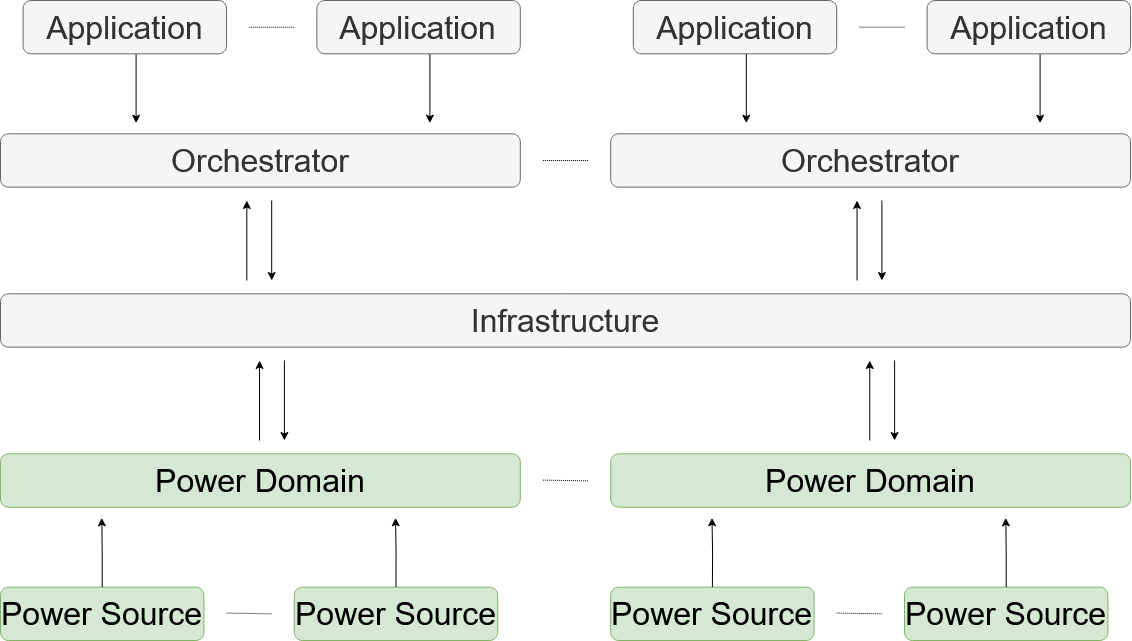
\includegraphics[width=0.9\textwidth]{images/Architecture.pdf}
    ~
    \caption{Architecture overview showing interactions between layers.}
    \label{fig:archtecture}
\end{figure}

As we can see, similar to how the orchestrator class mediates the relationships between the application and infrastructure layer, ECO-LEAF allows interactions to occur between the power source and infrastructure layer through power domains.

\section{Fundamentals of ECO-LEAF}
The following subsections go on to discuss the fundamental concepts used in developing ECO-LEAF, cover the ideas and techniques that are common throughout the framework and act as to how the simulation can take place.

\subsection{Discrete Event Simulations}\label{imp:subsec:des}
As briefly mentioned in Section \ref{subsec:power-domain-workflow} LEAF and subsequently ECO-LEAF forward time through DESs.
ECO-LEAF incorporates this through the use of the Python SimPy package \citep{simpy}.
Looking at Listing \ref{lst:simpy} we can provide an example to show how the SimPy package can create a simulation instance and execute code periodically:
\begin{lstlisting}[language=python, numbers=left, caption={Example use of the SimPy environment}, label=lst:simpy]
    def driver_Method():
        env = simpy.Environment()
        env.process(task(env))
        env.run(until=10)  # Run simulation for 10 units of time

    def task(env):
        while True:
            current_time = env.now()
            print(f"Task has been ran at time increment {current_time}")
            yield env.timeout(2)

    driver_Method()  # Run driver method
\end{lstlisting}
\begin{lstlisting}[language=TeX, caption={Terminal output of Listing \ref{lst:simpy}}, label=lst:simpy-output]
Task has been run at time increment 0
Task has been run at time increment 2
Task has been run at time increment 4
Task has been run at time increment 6
Task has been run at time increment 8
\end{lstlisting}

In this, we can see that the Environment() class is used to declare and initialise the simulation, keeping a reference to the env variable.
The example then informs the model to execute the task method inside the simulation environment by invoking process() with the task method call passed as a parameter.
Finally, the simulation's terminating condition is defined by passing an explicit value for the until argument, signalling that the simulation will terminate when the simulation's internal clock equals 10.
To allow the task method to be considered an `event' by the SimPy environment, it must be considered a ``Python generator'', where the yield environment.timeout() is inside the body of the method to allow the state of the model to progress forward in time.
In order to allow for the task to be called periodically, the task method encloses the logic of its body inside an indefinite while loop and uses yield environment.timeout(2) to pause the simulation for two units of time.
Fundamentally, ECO-LEAF uses this approach to allow the power domain to execute its workflow on the model's most current state during the simulation.

\subsection{Time}\label{imp:subsec:time}
Now that we have explained how ECO-LEAF uses SimPy to facilitate DESs and can progress the model forward in time, we can discuss how and why the implementation does this.
As a consequence of the implementation using historical data that is associated with an exact 24-hour time, \textit{the topic discussed in the upcoming section}, ECO-LEAF needs the means to go from an integer-based representation of time to one that is formatted as HH\%MM\%SS.
This is achieved by having the simulation assume that for every increment of 1 in the simulation's internal clock, a minute or 60 seconds passes inside the environment space.
A minute was chosen because the simulation could avoid taking unnecessary measurements of the simulation for small periods where the model's state is unlikely to change but still capable of capturing changes in the state that would only occur in a relatively short period.
However, in simulations that execute for periods longer than 24 hours (1440 seconds), it is still necessary to allow the simulation to identify the current state uniquely, something that cannot occur when time is represented as HH\%MM\%SS. Therefore, ECO-LEAF identifies the current state of a simulation at any given moment by using the clock's internal representation through env.now(), as any changes in the current state cause the time to progress within the simulation space.
This ensures that when data is written to a file, entries logged by the power domain will not get overwritten as they both uniquely represent the same time.

\subsection{Accessing Data}\label{imp:subsec:daa}
A core requirement of the project was to allow for fluctuations in PA. ECO-LEAF models a power source's PA and CI as values that are updated every step forward in time.
When the simulation moves forward in time, a power source will determine its available power and carbon intensity that it should have at that corresponding moment.
For cases where PA fluctuates (power sources that are not assumed to have a constant rate of power generation), the power source will consult a dictionary of corresponding (time, power) pairings using the current time of the simulation to produce the key to determine its power.
This data is loaded from a formatted CSV file when the class is initialised and provides data for 24 hours, where mechanisms within ECO-LEAF return to the start when the end has been reached.
Because the original datasets differed in the rate at which measurements of power throughput were captured, there are discrepancies in time granularity for when a power source sees a change in available power.
For instance, one data set that fluctuates aggressively may have a reading every minute to capture this property.
In contrast, a power source with reasonably minimal changes in power may only have readings every 30 minutes.
To resolve this, ECO-LEAF assumes that between changes in power readings, the power source maintains the previous rate until a new value can be retrieved.
This can be seen in Listing \ref{lst:time} which demonstrates how this assumption is implemented.\\

\begin{lstlisting}[language=python, numbers=left, caption={Example use of how a power source accesses it's available power.}, label=lst:time]
    def get_power_at_time(self, time_int) -> float:
        time = self._map_to_time((time_int // self.update_interval) % len(self.power_data))
        return float(self.power_data[time])
\end{lstlisting}

In order to find the appropriate key to determine the PA, the method carries out a floor division between the current time and the difference in time between readings to find the most recent time.
The implemented mechanism that allows simulations to occur for periods longer than 24 hours operates by wrapping the current time key back to the start of the data.
This is done by applying the modulus of the dictionary's size to this value.
From this, \_map\_to\_time() is used to convert this integer representation of time to a 24-hour string key to obtain the correct power from the dictionary.
To help illustrate this idea, Table \ref{tab:data-dic} visualises the first ten minutes of a potential example dictionary.
Table \ref{tab:time-explanation} describes how this data describes the first 10 minutes of this power source's availability.
\begin{table}[h]
    \rowcolors{2}{}{gray!3}
    \caption{Table depicting the data held in the file.}
    \label{tab:data-dic}
    \centering
    \begin{tabular}{@{}ccc@{}}
    \toprule
    \textbf{Time} & \textbf{Power} \\
    \midrule
    12:00:00      & 102            \\
    12:05:00      & 114            \\
    12:10:00      & 127            \\
    \bottomrule
    \end{tabular}

    \vspace{1em} % Add some vertical space between the tables
    \rowcolors{2}{}{gray!3}
    \caption{Table depicting how in reality power would be read from a power source's dictionary}
    \label{tab:time-explanation}
    %\tt
    \begin{tabular}{@{}lll@{}}
    \toprule
    \textbf{Env.now()}    & \textbf{Key}       & \textbf{Power}     \\
    \midrule
    0                     & 12:00:00           & 102                \\
    1                     & 12:00:00           & 102                \\
    2                     & 12:00:00           & 102                \\
    3                     & 12:00:00           & 102                \\
    4                     & 12:00:00           & 102                \\
    5                     & 12:05:00           & 114                \\
    6                     & 12:05:00           & 114                \\
    7                     & 12:05:00           & 114                \\
    8                     & 12:05:00           & 114                \\
    9                     & 12:05:00           & 114                \\
    10                    & 12:10:00           & 127                \\
    \bottomrule
    \end{tabular}
\end{table}

\section{Providing Power and Calculating Carbon Emissions}

\subsection{The Power Domain}\label{sec:power-domain}
The power domain is implemented in ECO-LEAF through the class type of PowerDomain.
To introduce the power domain within the simulation space, the user must initialise an instance of the class and pass an instance of its run method into the environment.
When initialising an instance, the user configures the power domain by passing through these items:
\begin{itemize}
    \item \textbf{env}, this is the reference to the Environment() class used to simulate the model.
    \item \textbf{name}, the name of the power domain. This value must be unique as it identifies the power domain.
    \item \textit{(Optional)} \textbf{start\_time\_str}, this is the string time for when the simulation should start. \textbf{powered\_infrastructure}, these are the entities the user wants to immediately assign to a power source dynamically.
    \item \textit{(Optional)} \textbf{powered\_infrastructure\_distributor}, the custom entity distribution method. NB, this replaces the default implementation provided by ECO-LEAF.
\item \end{itemize}

\subsubsection{Utility Functions}\label{imp:subsec:utility}
As the power domain is the focus of the features provided in ECO-LEAF, the class provides an array of methods that allow the workflow to carry out its tasks.

When a power domain is initialised, it may have been apparent that no power sources are passed through the constructor argument;
this is because the first feature provided by the power domain is add\_power\_source(), which creates these associations between a power source and a power domain().
When the power domain invokes add\_power\_source(), the power source's priority is used to insert the power domain into the correct location within the power domain's list data structure power\_sources.
When a power domain no longer wishes to associate with a power source, it invokes the instance method remove\_power\_source ().
This is to ensure that the power source is correctly removed from the power domain and that any entities currently powered by it are safely removed.
Adding and removing power sources allows users to describe scenarios where a power source may become available or unavailable during the simulation;
this could potentially model external factors such as power cuts.

The power domain's following core utility function is the ability to create and remove associations between infrastructure entities and the power domain.
The power domain achieves this by calling add\_entity() and remove\_entity(), respectively.
Similar to those for the power sources, add\_entity() and remove\_entity() safely add and remove infrastructure entities to the power domains list structure powered\_infrastructure.
This feature could be useful by considering the proposed events system, where the dynamic mobility of entities within the network allows them to move from one power domain to another. For instance, a mobile phone is being charged at one site and then another.

The final core feature of the power domain is the function used to calculate the amount of carbon produced.
As a core goal of the project was to introduce this ability, it was critical to provide this feature somewhere accessible to most classes.
Listing \ref{lst:calc-carbon} shows that the class function takes as arguments the energy consumed (in watt-hours) and a power source's current carbon intensity to calculate the amount of carbon released.
\begin{lstlisting}[language=python, numbers=left, caption={Listing showing the class method used to calculate carbon emissions.}, label=lst:calc-carbon]
    @classmethod
    def calculate_carbon_released(cls, power_used, carbon_intensity) -> float:
        return float(power_used) * (10 ** -3) * float(carbon_intensity)
\end{lstlisting}

Finally, the power domain also provides various small class functions to carry out common tasks, for instance, convert\_to\_time\_string() and get\_current\_time().

\subsubsection{Workflow}\label{imp:subsec:workflow}
As discussed in Section \ref{subsec:power-domain-workflow}, the workflow of the power domain is where the main interactions between the Power and Infrastructure layers occur.
ECO-LEAF implements this workflow by providing an invokable run method for an instance of the PowerDomain class.
Using the ideas presented in Section \ref{imp:subsec:des}, this method is passed through into the simulation environment to progress the simulation forward in time.

The power domain combines tasks in the workflow into the same body of a for loop when possible to minimise iterating through the power sources multiple times.
In addition, the power domain takes advantage of the ordering of its power\_sources list. It uses this to iterate through each power source, as the source's priority determined the position within this list when the power source was added.

The first for loop iterates through power\_sources in order to define each power source's available power and carbon intensity at that moment in the simulation.
This is necessary before the next for loop, as the distribution process in the following stage considers the power and carbon intensity of other power sources. Therefore, these must be updated before the following stages occur.

Once all the power sources have their values updated, each power source determines the infrastructure entities it will power for the current time step and log its measurements.
We can take measurements at this stage because ECO-LEAF iterates through power sources in the order of most desirable as explained in \ref{subsec:distributing-entities}.
Because of this, once a dynamic power source receives its allocated entities from the power domain, these entities will remain there until time moves forward.
For static power sources, rather than receive entities through the distribution method, evaluate those with a constant relationship.

Finally, the workflow evaluates whether all entities possess an association with a power source; if this is not true, the simulation fails by raising an error.
\subsubsection{Distributing Entities to Power Sources}\label{imp:subsec:distributor}
The power domain uses the PoweredInfrastructureDistributor class to distribute entities within the infrastructure to power sources.
The class contains only two attributes:
\begin{itemize}
    \item \textbf{powered\_infrastructure\_distributor\_method}, this is the method which determines entities for a given power source.
    \item \textbf{smart\_distribution}, this is used within the default method to allow for advanced features.
\end{itemize}
The class is initialised in one of two ways: letting the framework initialise a default implementation or creating a custom instance with a custom distribution method.

For context, when a power source evaluates an entity, an inequality comparison is carried out between the power source's available power and an entity's power requirements.
When the power domain calls the distributor method, it passes in two items: the power source which wants to receive entities and the power domain itself.
The method receives the power domain in order to see the entities within it.
The method then selects and returns the most appropriate entities for a given power source.

As defined in Section \ref{subsec:distributing-entities}, the entities are separated into three categories.
The first category evaluated is the entities that the power source powered in the previous state of the simulation.
It evaluates these first as the system assumes that these should try to retain an association before distributing power elsewhere.
If the source can no longer power one of these entities, the entity the power source removes it from its list of powered\_infrastructure.

After this, the method evaluates entities that have no power source.
It evaluates these entities second, as the simulation would fail if an entity could not be assigned a power source.
If an entity here can join the power source, the method adds the entity to the power source's powered\_infrastructure.

Finally, the method uses the instance's smart\_distribution attribute and the current power source's priority to try to power entities from less desirable power sources.
This process occurs last because the categories above take more precedence over this one.
If an entity can join the power source, it is first removed from the previous power source's list of powered\_infrastructure and added to its own.

\subsubsection{Logging Results}\label{imp:subsec:logging-results}
The power domain implements the ability to record measurements about the simulation's current state by building a nested dictionary as it moves forward in time.
The benefit of working with nested dictionaries is that this can be easily transformed into a JSON file to write a file later on, and amendments can be made when appropriate.
Appendix \ref{lst:dic-log} shows an example of this tree-like structure.
The results of the simulation are structured hierarchically.
The outer dictionary contains information about the entire simulation.
The next level describes the state of the environment at any given moment.
The layer after this defines the current state of each power source.
Finally, the innermost state describes the measurements of the entities.
By organising items in the simulation this way, the power domain eliminates the need to explicitly describe associations, reducing redundancy and the size of results.
The listing shows that the dictionary's power source level also describes particular attributes of the power source.
This is done to keep a record of the power source at that moment during the simulation's runtime.
These values can later be used when analysing results.

\subsection{Power Sources}\label{sec:power-sources}
Power sources are implemented in ECO-LEAF using an abstract class to define the class instances' universal attributes and methods.
By using abstract classes, the user can focus on defining the logic unique to a particular power source without having to consider implementing the functionality already defined in the abstract class.
Because the power domain only considers a few abstract methods, the effort required to develop custom implementations of power sources is minimal.
As discussed in Section \ref{sec:power-sources}, power sources are classified through two distinct features: their type and whether they are static or dynamic power sources.
The power type of a power source is implemented through an enumerator to describe the three potential types that exist: RENEWABLE, MIXED and BATTERY.
If the user wishes for a power source to maintain a constant relationship with a collection of entities, then the static argument must be set to True in the constructor along with providing the entities they wish to have an association.\\
ECO-LEAF initialises power sources by defining a concrete instance of the PowerSource class.
These instances are designed to simulate the characteristics of the power sources they are based on.

While the user can develop their own power sources, ECO-LEAF provides four main examples: Solar Power, Wind Power, Grid Power, and Battery Power.
These power sources take from real-life historical data to define their behaviour in each state of the simulation.
For instance, renewable power sources (SolarPower and WindPower) retrieve data for their PA (with the default data being provided from EirGrid \citep{eirgrid}), whereas non-renewable power sources (GridPower) retrieve data for their carbon intensity (with the default data being provided from the Carbon Intensity API \citep{carbon_intensity_api}).
Finally, the BatteryPower class is unique, as it stores power rather than generates it.
This source acts differently and only updates naturally to return to full power once another power source charges it.
Suppose the user wishes to implement their own power source.
In that case, they are expected to define the logic for updating and providing information about the current PA and the carbon intensity at that moment in time.

Power sources provide the user the ability to configure them in a variety of ways.
The user achieves this through the arguments they provide during the initialisation of the instance:
\begin{itemize}
    \item \textbf{env}, the reference to the Environment() class used to simulate the model.
    \item \textbf{name}, the name of the power source, like the power domain, must be kept unique as it is used to identify itself.
    \item \textbf{data\_set\_filename}, this is the file path for the data that fluctuates: either the carbon intensity or available power.
    \item \textbf{power\_domain}, this is the power domain instance. NB, this is required to acknowledge the time the simulation starts.
    \item \textbf{priority} is the integer that describes preference when distributing entities where 0 is the most important.
    \item \textit{(Optional)} \textbf{static}, this is a boolean flag to signal to the power domain, not to distribute entities to this power source.
    \item \textit{(Optional)} \textbf{powered\_infrastructure}, these are the entities the user wants to assign to a power source statically.
\end{itemize}
The PowerSource class represents the available power at any given moment in time by using a floating point variable \textit{remaining\_power}.
While \cite{leaf2021} use a power model in the Application and Infrastructure layer to represent static and dynamic power consumption, ECO-LEAF only needs a single value.
To convert from a PowerModel reading of power to a single value, the power domain casts the type as a float to retrieve the required power.

\subsubsection{Evaluating Entities within Static Power Sources}\label{imp:subsec:static-entities}
While the PoweredInfrastructureDistributor class distributes entities to dynamic power sources, static power sources also need to determine what entities they will power at each moment in the simulation.
Because of this, the power source provides a crucial method called \textbf{evaluate\_entities}.
The purpose of this method, \textit{just like the powered\_infrastructure\_distributor\_method}, is to determine which entities are powered at the current state of the simulation for static power sources.
It achieves this by iterating through each entity present and carrying out the same evaluation discussed in Section \ref{imp:subsec:distributor}.
However, as the power source is considered static, the method cannot simply free the entity back to the power domain for another power source to power.
Instead, the power source effectively turns off the entity by pausing it and removing any tasks or dataflows in the entity itself and the remaining application.

\subsubsection{Functionality}\label{imp:subsec:utility-funcs}
Like the PowerDomain class, the abstract class of PowerSource provides the user with a range of functions available to all realised instances of the class.
Unlike the abstract methods, which are specialised to each individual concrete class of PowerSource, these methods provide the same functionality throughout all instances.

The first collection of functions the PowerSource class provides is related to power consumption.
These include providing safe approaches in consuming (\textit{consume\_power()}), setting (\textit{set\_current\_power()}) and retrieving power (\textit{get\_current\_power()}).
Because of this, when the simulation needs to interact with the current remaining power of a power source, they can call these methods without worrying about providing checks to ensure correctness.
The PowerSource class also provides essential add and remove methods to include and drop entities from within their list of powered\_infrastructure.
Similar to the PowerDomain class, these add and remove methods correctly ensure that when an entity is handled by the power source, the necessary processes have occurred to prevent entities from not being correctly updated.

Finally, the PowerSource class is also responsible for processing the data regarding the particular power source instance.
In addition, the method processes the data to start at the user's desired time, allowing users to define when a simulation can start without having to move the simulation's internal clock forward to achieve this.

\section{Events}\label{imp:sec:envts}
ECO-LEAF implements events in the framework by introducing Event and EventDomain classes.
Similar to the definition used to describe events in DESs \citep{Des}, an Event instance in this context describes a method that will be executed at some point during the simulation.
An instance of EventDomain manages these events and moves independently within the simulation, executing them when appropriate.

\subsection{Events}\label{imp:subsec:event-class}
The Event class aims to inform an instance of EventDomain how and when to execute a callback method.
Because of this, the class provides no functionality besides being initialised.
An event is described through the following attributes:
\begin{itemize}
    \item \textbf{event}, this is the method the user wants to execute. NB, the user should only reference the method; therefore, no parentheses are included.
    \item \textbf{args}, this is a list of the arguments that must be passed into the method.
    \item \textbf{time\_str}, this is the (string) time when the event should execute. NB, this should be formatted as HH\%MM\%SS.
    \item \textit{(Optional)} \textbf{repeat}, this is a boolean flag to signal whether the event should execute after a certain amount of time has elapsed.
    \item \textit{(Optional)} \textbf{repeat\_counter}, following from repeat, this indicates how much time should elapse in minutes before the event executes again.
\end{itemize}

\subsection{Managing Events}\label{imp:subsec:event-domain-class}
As previously mentioned, the goal of the EventDomain class is to manage when events are executed within the simulation.
Just like the Event class, the EventDomain instance is expected to be initialised by the user by considering the environment (env), the amount of time elapsed between considering events (update\_interval) and the time the manager starts running (start\_time\_str).

When the user defines the simulation model, instances of the Events class are associated with the event domain by calling the add\_event() method.
Like the PowerDomain class, the EventDomain moves independently within the simulation space using the same approach outlined within Section \ref{imp:subsec:time}, where a driver method is used to iterate constantly through time within the simulation.
When the event domain does move forward in time, the driver method calls the only other method available run\_events().

The run\_events() method operates by first finding the current time of the simulation and initialising an empty list.
The purpose of this list is to identify any events that have been executed during this time interval of the simulation so they can be safely removed afterwards.
The method then proceeds to iterate through its events.
During this, each event is evaluated using an inequality comparison.
If the current time equals or surpasses an event's execution time, the event's method is called passing in any provided arguments.
If the user wishes for an event to be repeated and executed regularly, a new event instance is created by copying over the attributes of the old event, with the execution time incremented.
After this, the event is added to the event\_history list data structure to log executed events.
Finally, the old event is flagged and ready to be deleted once all other events have been run.

\section{Results}\label{sec:displaying-results}
The final aspect introduced into ECO-LEAF is the ability to store and display results.
Using the data logged from Section \ref{imp:subsec:logging-results} ECO-LEAF allows the data generated during the simulation to be saved to a file and visualised through graphs and animations.
It achieves this by using the Python packages Plotly \citep{plotly-git}, Matplotlib \citep{Hunter:2007} and NetworkX \citep{networkx}.
Once the simulation has finished executing, the user is free to analyse the data however they deem fit.
ECO-LEAF provides the user with three classes to view the data:

\begin{enumerate}
    \item FileHandler
    \item FigurePlotter
    \item Animation
\end{enumerate}

\subsection{File Handling}\label{subsec:imp:filehandler}
The FileHandler class saves writable objects to a file.
Similar to the native FileHandler class in Python \citep{python-docs-FileHandler}, the FileHandler class in ECO-LEAF provides the necessary features to write both the power domain's results of the simulation and any graphs generated to the file.
It achieves this by creating a unique directory within the results folder. The folder's name reflects the file from which the FileHandler was initialised, along with a date and time stamp.
If the user wants to use the class, they are expected to initialise an instance.
This class was implemented to keep the user's focus of ECO-LEAF on creating simulations rather than dealing with file writers.

\subsection{Plotting Graphs}\label{subsec:imp:figureplotter}
The user can generate automated graphs of the simulation by utilising the FigurePlotter class.
This class's goal is to provide a collection of functions that can be used to generate instances of Plotly.Figure.
If the user wants to use this class, then an instance of it must be initialised by passing through the following items:
\begin{itemize}
    \item \textbf{power\_domain}, the power domain from which the user wants to produce results.
    \item \textit{(Optional)} \textbf{event\_domain}, the event domain that issued any events in the same simulation space as power\_domain.
    \item \textit{(Optional)} \textbf{show\_event\_lines}, this is a boolean flag for a stylistic choice to have lines that intersect events cut through other figures.
    \item \textit{(Optional)} \textbf{(number\_of\_divisions)}, this is an integer used to indicate how many x-ticks there should be.
    \item \textit{(Optional)} \textbf{title}, this is the overall title if an aggregated figure is used.
\end{itemize}
Once an instance has been defined, the user can invoke the instance and generate a figure by calling any of these methods:
\begin{itemize}
    \item subplot\_time\_series\_entities()
    \item subplot\_time\_series\_power\_sources()
    \item subplot\_time\_series\_power\_meter()
\end{itemize}
By passing through the desired attribute and necessary instances to plot, the methods return an instance of Plotly.Figure.\\
Finally, the class can reduce the number of figures present by aggregating the graphs into the same figure and converting the existing figure into sub-figures.

\subsection{Animating Results}\label{subsec:imp:animation}
The last major class ECO-LEAF saw to provide was a means to visualise how infrastructure entities interacted with power sources during the simulation.
This class was needed during development to evaluate the examples produced alongside the framework, as having textual descriptions of relations in the debugger used did not provide enough detail about how entities were being distributed among power sources.

The Animation class achieves this by providing an interactive means to move through each simulation state and view the relations between entities and power sources.
It implements this using the Matplotlib and NetworkX packages to place a series of graphs over an interactive plot.
When the play button is pressed or the slider moves across the time series, a new NetworkX graph is generated.
When this happens, an index of that current moment is used to generate the relationships that existed by inspecting the corresponding entry in the power domains log using the key values to decide.
Figure \ref{fig:dev-example7-animation} shows an example instance of this animation.
\begin{figure}[h]
    \centering
    \includegraphics[width=0.50\textwidth]{images/example7-animation.pdf}
    ~
    \caption{Example figure generated from 7\_extended\_file\_writer.py in the development\_examples folder.}
    \label{fig:dev-example7-animation}
\end{figure}

%==================================================================================================================================

\chapter{Evaluation} \label{chp:evaluation}
%How good is your solution? How well did you solve the general problem, and what evidence do you have to support that?

\section{Experimental Setup}\label{eval:sec:scenarios}
To determine whether the goals laid out for ECO-LEAF in Chapter \ref{chp:intro} were met, various scenarios have been developed under the context of a farm located in Northern Ireland that utilises precision agriculture.
Northern Ireland was chosen due to its variability in short-term weather and accessibility to public records about energy generation statistics.
Throughout the chapter, the evaluation will cover particular scenarios that effectively demonstrate the features proposed in ECO-LEAF.
Using the goals as a reference, scenarios will identify when and why a particular goal has been met.
The scenarios were designed to slowly introduce fundamental concepts of ECO-LEAF before moving on to more advanced examples.
While not all scenarios could be evaluated to ensure that enough detail was given to those that were, all diagrams and results will be attached as appendices.

\subsection{Precision Agriculture}\label{eval:subsec:precision-agriculture}
Precision agriculture, also known as smart farming, is a farming technique that uses technology and data processing to optimise the various aspects of production in agriculture.
The practice intends to use data analytics to increase efficiency, sustainability, and productivity compared to traditional farming practices \citep{precison-agriculture}.
It achieves this by encompassing a range of techniques such as precision crop management, remote sensing, and automated machinery.
By using autonomous equipment to capture and react to information about the current landscape, the site-specific needs of a farm can be met, allowing for equal or larger yields whilst reducing their consumption of resources during the process \citep{precison-agriculture}.
The practice can be represented in three main stages: Data capture, Interpretation, and Application.
Data capture involves measuring and recording aspects of the local environment, such as capturing the moisture and pH of soil.
Interpretation involves aggregating and processing the raw data before determining a plan of action.
Finally, Application occurs to carry out these actions; this can be an automated or manual process.

As precision agriculture utilises large-area data capturing and analysis, a network infrastructure is required to provide communications between sensors and processing services.
Because of this, fog computing networks are able to be utilised to improve the sustainability of the practice \citep{fog_smart_farming}.

\subsection{Defining Models}\label{eval:subsec:modelling}

\subsubsection{Applications}
Applications represent the first two stages of precision agriculture: Data Capture and Interpretation.
They describe streams of data being captured by sensors, which then travel to fog nodes for pre-processing before finally being handled by the cloud.
Application tasks are modelled with pseudo-arbitrary values that consider the current stage of precision agriculture it is in.

As LEAF allows for the CU of devices to be defined in any context, rather than use MIPS as discussed in Section \ref{leaf}, CU will be considered a generic value for computing load.
This can occur as the accuracy of these values is irrelevant in the context of evaluating the aims of the project.
As such, a task's required CU will represent a ratio of CU needed to carry out the current stage of the application.
The Capture stage is represented as the sink task, its required CU reflects the hardware they run on in order to capture measurements.
The interpretation stage is represented through processing and sink tasks, where the combined CU of all these tasks should equal 200.

Source tasks are modelled to consume 90\% of a sensor's computational load.
As the sensor's primary goal is to take continuous measurements, the task can therefore consume most of the sensor's resources.
Processing tasks are modelled to consume a static 50 CU (12.5\% of a fog node's computational load).
As the scenarios only consider one type of fog node this value will remain at 50.
Finally, sink tasks as a result, model their CU ($CU_{server}$) through the formula $CU_{server} = 200 - (n \times 50)$ where n is defined as the number of processing tasks in an application.
As the Interpretation stage of the application requires 200 CU, a sink task is required to carry out the remaining computations needed to process the data.


\subsubsection{Infrastructure}
Network topologies in the scenarios can consider four types of devices: Sensors, Drones, Microprocessors, and Servers.
For the sake of simplicity, links are provided with no power model, to keep the focus on interactions with nodes, and can either represent a wireless WAN connection with a bandwidth of 30Mb/s or a wired connection with a bandwidth of 50Mb/s.

A sensor describes the stationary devices that capture measurements about the farmland.
The power model for sensors is based upon the requirements for the 6345CSOV Leaf and Soil Moisture/Temperature Station provided by \cite{prodataWeatherSystems}.
The CU for a sensor is defined as 10 CU.
In this context, drones are considered to be mobile end devices. While they will not be used until the final scenario, their model descriptions will be provided here.
The drone power model is based upon the Matrice 300 RTK aircraft supplied by \cite{drone_spec}.
As drones capture visual information about the farmland, their CU is set to 30 to reflect this.

Microprocessors describe the fog nodes for the simulation, the fog node aims to alleviate computational demand from the server by preprocessing the data before arriving there.
The microprocessor power model is based upon a Raspberry Pi 2 B with external USB 3.0 SSD \citep{pidramble}.
Utilising such a power model, in comparison to what may be used in other scenarios, is necessary because the data being captured does not require computationally powerful hardware to preprocess the applications.
Microprocessors use a CU of 400.

Finally, servers describe the cloud computing devices of a fog network. Their goal is to aggregate and process the data captured in the simulation.
As servers will be processing vast amounts of data, their power models will not consider a max power requirement and instead consume energy based on their current CU, using a rate to convert this to power.
This value will be set to 20mW/CU because the value itself is irrelevant as long as it is used consistently throughout the evaluation.
\subsubsection{Power Sources}
Finally, solar, wind, battery, and national grid power sources are used throughout the scenarios.
For solar and wind power, as the context considers a theoretical farm located in Northern Ireland, their power models retrieve historical datasets from \cite{eirgrid}.
To model their CI, scenarios consider them static at 46 and 12 gCO2eq/kWh, respectively.
These were retrieved by considering the life cycle assessment of their technologies from the \cite{ipcc_synthesis_2014}.
When modelling grid power, we assume that power generation is infinite and CI fluctuates due to the heterogeneous nature of the energy mix.
This is modelled using the historical data set provided by the Carbon Intensity API \citep{carbon_intensity_api}.
Finally, for battery power, only the available capacity of the device needs to be considered.
As the context of the battery varies from scenario to scenario, the value will be discussed when appropriate.
\clearpage

\section{Scenario 1 - A Singular Static Power Source}\label{eval:subsec:scenario1}
Scenario 1 provides the simplest use case of ECO-LEAF and defines a static grid power source with a sensor, microprocessor, and server connected together.
A single application runs on top of this, with the simulation lasting 11 minutes.
The goals explicitly demonstrated here are 1.1, 1.2, 2.1, and 2.2.
The aim is to show that entities within the infrastructure are allocated power and produce carbon emissions due to consuming this energy.
Figure \ref{fig:example1_diagram} in the appendices illustrates how the power, infrastructure and application layers interact.
\subsection{Scenario 1 Results and Analysis}
\begin{figure}[h]
    \centering
    \includegraphics[width=\textwidth]{images/examples/example_1/energy_usage_1}
    ~
    \caption{Graphs showing energy usage throughout the simulation of scenario 1. For the full results please refer to Appendix \ref{apen:subsec:scen1}.}
    \label{fig:example1_results_energy}
\end{figure}
Looking at Figure \ref{fig:example1_results_energy}, we can see that despite the basic nature of the scenario, Graphs 1.1 and 1.2 indicate that the correct amount of energy is being consumed from the power source.
This can be seen as, at any given moment, the energy consumption for entities in Graph 1.1, when summed, equal the corresponding energy provided by the grid power source in Graph 1.2.
The same relationship can also be seen in the carbon released for Graphs 1.3 and 1.4 in the appendices.
This can be explained with the equation for carbon released defined in Section \ref{subsec:carbon-released}.
As power and carbon emissions produced are proportional to one another, the carbon released is a scalar value of power consumed.
Because of these results, goals 1.1, 1.2, 2.1, and 2.2 have all been met, as power sources can supply energy to network infrastructure and, as a consequence, produce carbon emissions.

\section{Scenario 3 - A Custom Infrastructure Distributor}\label{eval:subsec:scenario3}
Scenario 3 is designed to showcase the infrastructure's capability to assign nodes to different power sources, thereby fulfilling goals 1.3, 1.5.
In the simulation, solar, wind, and grid energy sources are utilised, being preferenced by the power domain in the same order.
The simulation runs between the time 7pm and 8pm.
In addition to the normal allocation process, the custom distribution method also assigns nodes with no max power requirement to power sources with infinite PA.
To see these changes, while the scenario's topology remains the same, the server's power model is modified to no longer consider a maximum power requirement.
As such, the simulation results should show that despite grid energy being the least desirable, the server only receives power from this source while the sensor and microprocessor dynamically change power sources as the environment's state evolves.
Figure \ref{fig:example3_diagram} illustrates an overview of the scenario.
\begin{figure}[h]
    \centering
    \includegraphics[width=0.8\textwidth]{images/examples/example_3/example3_diagram.pdf}
    \caption{Illustration depicting scenario 3.}
    \label{fig:example3_diagram}
\end{figure}

\subsection{Scenario 3 Results and Analysis}
Figure \ref{fig:example2_switch} displays the connections between various power sources and the infrastructure at two different times - 7pm and 7:30pm.
This figure was created by capturing individual frames from the animation tool provided by ECO-LEAF.
At 7pm, we can see that the distribution method successfully supplied power to all entities in the infrastructure.
As expected, all devices were running on solar power except for the server, which was connected to the grid.
At exactly 7:30 pm, the distributor method correctly switched renewables and dynamically distributed power from the wind power source as the solar supply could no longer provide enough energy.
However, as the links do not consume energy we still see associations between them and the solar power source.
This can also be seen in Figure \ref{apen:scen3} as Graph 3.2 depicts the energy provided by power sources throughout the simulation.
As expected, the desired characteristics can be seen: Grid power provided a consistent amount of energy (indicating that it always provided power to the server), solar power provided power up until 19:30:00 (as it could no longer generate power from the sun), and finally wind power (as the second most preferable power source) started to provide power once solar could no longer do so.
Because of this, ECO-LEAF achieves goals 1.3, 1.5.
Specifically, we see the solar power source fluctuate in PA as a consequence of time and that the power domain dynamically distributes infrastructure to other power sources.
\begin{figure}
    \centering
    \includegraphics[width=0.85\textwidth]{images/examples/example_3/switch}
    \caption{Graphs showing associations between infrastructure and power sources at the start of the simulation and 30 minutes through. For the full results please refer to Appendix \ref{fig:example3}.}
    \label{fig:example2_switch}
\end{figure}

\section{Scenario 5 - A Carbon Aware Application Orchestrator}\label{eval:subsec:scenario 5}
Inspired by Cucumber \citep{cucumber}, Scenario 5 aims to consider the deployment of applications over infrastructure by considering the CI of available power sources.
As such, the scenario aims to demonstrate goal 2.3 by allowing users to consider power sources when placing applications on infrastructure.
It aims to achieve this by evaluating the number of processing tasks and the current CI of power sources.
As tasks cannot switch between infrastructure on their own, the scenario utilises the Events class to periodically place applications on devices and then subsequently remove them after a period of time.
In the scenario, this describes sensors taking measurements and idling for 10— and 30-minute intervals between 2 pm and midnight.
The scenario uses static solar, grid, and battery power sources as we wish to only evaluate the placement of applications on the infrastructure.
As application placement now considers the number of tasks and the power source used, the scenario utilises two applications and defines a new network topology.

\begin{figure}[h]
    \centering
    \includegraphics[width=0.72\textwidth]{images/examples/example_5/example5_diagram.pdf}
    ~
    \caption{Illustration depicting scenario 5.}
    \label{fig:example5_diagram}
\end{figure}

Application 1 (A1) is the application used in previous scenarios, Application 2 (A2) is an application that contains two processing tasks.
A new topology has been designed to consider one sensor, three fog nodes and one server.
The exact structure of the network can be seen illustrated in Figure \ref{fig:example5_diagram}.
The goal is to demonstrate that the placement algorithm developed will always place an application on the infrastructure using the path with the smallest CIs.
For the sake of evidence, we will use the events mechanism to introduce the solar microprocessor at 4 pm, causing the simulation to transition from Config 1 to Config 2.
As such, the following characteristics should occur:
\begin{itemize}
    \item When the solar microprocessor is available, A1 should always follow the path outlined in config 2.
    \item When the solar microprocessor is unavailable, A1 should follow the path in config 1.
    \item A2 should always use the path containing the solar and battery microprocessors. This is because A2 always requires two microprocessors to run.
\end{itemize}

\subsection{Scenario 5 Results and Analysis}
\begin{figure}[h]
    \centering
    \includegraphics[width=0.75\textwidth]{images/examples/example_5/example_5_processors.pdf}
    ~
    \caption{Graphs showing the power consumed by the solar and grid microprocessors. For the full results please refer to Appendix \ref{fig:example5}.}
    \label{fig:example5_microprocessors}
\end{figure}

Both graphs in Figure \ref{fig:example5_microprocessors} show periodic rising and falling energy consumption as tasks are placed and removed from the devices, respectively.
As we can see in Graph 5.7, the energy consumption for the grid microprocessor occurs continuously for the entirety of the simulation, unlike that for the solar one, which is introduced at 4 pm and runs out of power at 8 pm.
Because of this, we can see the desired outcome from the application placement algorithm.
At the start of the simulation, we see Config 1, where A1 and A2 both have tasks that execute on the grid microprocessor, as there is no other available path to the server.
Once we see the solar power source introduced into the simulation, the solar microprocessor is available to run tasks.
Because of this, when A1's processing task is later deployed, the algorithm chooses the solar microprocessor as the CI for this power source is smaller than that of the grid.
Consequently, we see that the solar microprocessor now periodically runs the processing task, resulting in the results in Graph 5.6.
As the task is no longer run on the grid microprocessor, the amount of energy consumed falls, as seen in Graph 5.7.
Finally, at 8 pm, the solar power source no longer provides sufficient energy to its microprocessor.
This causes the model to revert to placing the application back onto the grid microprocessor, reflecting Config 1.
Because of this, we can claim that goal 2.3 has been met because the user is able to consider how applications are placed on the infrastructure as a consequence of power sources.

\section{Scenario 6 - Cyclic Infrastructure Pausing}\label{eval:subsec:scenario 6}
Scenario 6 is designed to demonstrate how applications and infrastructure can halt without power. This is to validate that ECO-LEAF meets goal 1.4, which states that power sources can only distribute power if it is available.
To demonstrate this, we consider two static power sources: grid and battery.
The simulation is run between 10 am and 8 pm, with the applications already deployed on the necessary devices.
Unlike previous scenarios, rather than utilising a single sensor in our network topology, in preparation for the final example, the simulation uses sixty.
The network is configured as shown in Figure \ref{fig:example6_diagram} where sensors are connected to their microprocessor until finally arriving at a single server.
Sensors and microprocessors have had their power models follow a Gaussian distribution for analysis purposes.
This was done to allow for a range in values for power usage across devices and is used to identify whether the scenario is working as intended.
In addition, power models have also been defined for links to consume 400nWh/bit. This has been done to later identify that infrastructure not powered by the battery remains powered throughout.
Sensors and fog nodes will be powered by a single battery source, while the server and links will be powered by the grid.
As the battery plays an essential role in the scenario, we configure the battery to have a total capacity of 15Wh.
At this capacity, the sixty sensors and microprocessors should be able to drain the available battery power multiple times.
While sixty fog nodes may be too excessive in a real scenario, as the aim here is to demonstrate power running out and microprocessors draw more power than sensors, we provide each sensor with its own rather than use more sensors to drain the power faster.

\begin{figure}[h]
    \centering
    \includegraphics[width=0.9\textwidth]{images/examples/example_6/example6_diagram.pdf}
    ~
    \caption{Illustration depicting scenario 6.}
    \label{fig:example6_diagram}
\end{figure}

As ECO-LEAF powers off infrastructure associated with a static power source rather than terminate the simulation when a device is unable to be powered, we should see that as the PA gets smaller and smaller, particular sensors and microprocessors should stop running until, eventually, no device can be powered.
As we see slight differences in power requirements despite running the same application, when energy availability gets low, rather than being unable to power all devices, those with smaller power requirements can still remain powered.
Because of this, devices with a higher energy demand should stop being powered first, followed by those with smaller requirements.

\subsection{Scenario 6 Results and Analysis}
Looking at Figure \ref{fig:example6_results}, we can see the two graphs: Graph 6.2, which shows the energy consumed by the infrastructure and Graph 6.6, showing the battery's remaining power.
It is important to note that the simulation predefined events at three points in time: 10:30 am, 2:30 pm, and 6:30 pm.
As we can see, before 10:30 am, nothing happens until the first event is called, as seen in Graph 6.3, which shows a significant spike in gird energy provided.
Once this occurs, the battery has enough power to turn on its devices and unpause their tasks.
We can see this through the microprocessors starting to consume energy.
While this happens over the next three hours, the battery consistently decreases in remaining power until it runs out just before 2 pm.
When this occurs, the battery starts to turn off all devices it can no longer power.
By 2:30 pm, all devices had been powered off. Here, the cycle repeats as the scheduled event charges the battery from the grid.
The results in Graph 6.3 clearly show how the battery and grid power sources provide energy throughout the simulation.
Because of this, we can see that ECO-LEAF can prevent devices from consuming power when none is available and, therefore, fulfilling the requirement of goal 1.4

\begin{figure}[h]
    \centering
    \includegraphics[width=0.75\textwidth]{images/examples/example_6/example_6_cutoff}
    ~
    \caption{Graphs showing the power consumed by the infrastructure and the energy available for the battery device. For the full results please refer to Appendix \ref{fig:example6}.}
    \label{fig:example6_results}
\end{figure}

\section{Scenario 7 - Precision Agriculture}\label{eval:subsec:scenario 7}
In this final scenario we explore a more realistic use case for ECO-LEAF in precision agriculture and determine whether goal 2.4 has been met.
This goal sees to ensure that the quantity of carbon emissions released can vary as a consequence of environmental conditions.
Because of this, the scenario explores the effect of running various combinations of power sources over identical parts in the network.
For context we will model the simulation environment as a farm.
This farm is simulated over a period of forty eight hours starting at 10 am, and considers four mostly identical plots of farmland.
These plots of land each cover 2500 square meters and depict the land used to plant crops.
In the simulation we again consider the Data Capture and Interpretation stages of precision agriculture.

The farm utilises two approaches in gathering data.
The first describes an array of sensors in a grid layout spaced evently throughout each plot.
In total each plot has 25 sensors.
In addition to this, each plot also employs a drone to travel across the land and carry out aerial surveying of the crops below them.
The drones flightpath takes it across the field in a row-major approach travelling across the plot before then proceeding to travel along it.
Thr drone uses a battery power source to provide power to fly along with running its application.
Once the flightpath has finished its flightpath, the drone goes to recharge.
Both the drone and sensors connect to a single fog node in the plot.

The fog node is situated at one corner of the plot and is the location the drone recharges at.
In order to accommodate all the computing required to handle the drone and sensors, the fog nodes computing CU is set to 1500.
The four fog nodes are then connected to the cloud.
The cloud connects all four plots together and is where all applications terminate at.
As the goal of the experiment is to explore how carbon emissions vary over these plots, each plot receives their own power sources.
The Plot 1 (P1) considers Solar, Wind, and Grid, Plot 2 (P2) considers grid and solar, Plot 3 (P3) considers only wind and finally (P4) considers just grid.
The setup for this scenario is depicted in Figure \ref{fig:example7_diagram}.

The expectation is that we should see all four plots run the same applications and as such power usage should be consistent.
However as different plots have different available power sources, we should see that plots that utilise renewables more should be greater than those that dont.

\begin{figure}[h]
    \centering
    \includegraphics[width=0.75\textwidth]{images/examples/example_7/example7_diagram.pdf}
    ~
    \caption{Illustration depicting scenario 7.}
    \label{fig:example7_diagram}
\end{figure}

\subsection{Scenario 7 Results and Analysis}
Looking at Figure \ref{fig:example7_final_results}, the graphs depict the accumulated carbon released throughout the simulation.
As expected, Plot 3 produced the least amount of carbon, followed by Plot 1, Plot 2, and finally, plot 4.

In Plot 3, only the wind power source has been utilised.
As the inherent CI of wind power is the smallest, it makes sense that the carbon released by this plot is also the smallest.
When looking at the carbon released for power sources in Graph 7.3.5 we can see a steady fluctuation in carbon released when sensor applications are placed and removed from the infrastructure.
This increases slightly at 11 am on both days because the drone's application is placed and transmits a constant stream of data during its flight to the fog node.
In addition, we can also see the drone's flight path through its energy consumption in Graphs 7.3.2 and 7.3.3 as spikes.
This is because the drone consumes energy to traverse the plot; the tallest spikes represent the drone travelling diagonally, as seen in Figure \ref{fig:example7_diagram}.
For all plots, we can see that the drone flies for a shorter period on the first day compared to day two; this is because the drone initially starts its flight path at the centre of the plot.

In Plot 1, solar, wind, and grid power sources have been used.
Looking at how carbon is released throughout the simulation, Graph 7.1.5 shows that Plot 1 only utilised solar and wind power.
This makes sense considering the carbon intensities and priority ranking of the power sources available to each plot.
As priority ranking precedes CI in ECO-LEAF, we can see that solar power is used more than wind when available.
As wind power has enough energy to power the entire infrastructure daily, despite being available to the plot, grid power in reality is never used.

In Plot 2, solar and grid power are used.
In Graph 7.2.5, we can see how both power sources were used throughout the plot.
As expected, we see relative lulls during the day as a consequence of solar power's ability to provide energy; when unavailable, the grid fulfils this energy demand.
Because of this, we see the opposite effect compared to Graph 7.1.5, as in this case, the CI for solar is much smaller than for grid.
At the start of the graph, we can see that the grid is also used to charge the battery.
The grid does this because solar does not have enough power to provide energy to the battery over the recharge time.
It's worth noting that relying solely on solar power was not feasible for any plot because of this.

Finally, in Plot 4, only grid power is used.
Because of this, looking at Graph 7.4.5, we can see that throughout the simulation, we can see oscillations in carbon released by the fog node as a consequence of CI gradually rising and falling throughout the day.
As we can see in Graph 7.0.4, grid has the highest CI at any time. Because of this, plot 4 produces the highest amount of carbon.

Overall, after carrying out analysis on the carbon emissions of various plots, scenario 7 clearly demonstrates how different environmental conditions can change the carbon released in the simulation.
Because of this, we can say that goal 2.4 has been met.\begin{figure}[h]
    \centering
    \includegraphics[width=0.55\textwidth]{images/examples/example_7/Main_results}
    ~
    \caption{Graphs depicting the timeseries of total carbon emissions for power sources. For the full results please refer to Appendix \ref{apen:scen7}.}
    \label{fig:example7_final_results}
\end{figure}

\section{Evaluation Overview}
To conclude the evaluation, the analysis of the scenarios indicate that the the goals outlined in Section \ref{intro:subsec:goals} have been achieved based on the individual criteria for each main goal being met.
From analysing the examples, it is clear that \textit{\textbf{(1) a means to model power sources}} was introduced into LEAF as a variety of power sources were modelled using ECO-LEAF and were used to provide power to infrastructure in the context of precision agriculture.
Furthermore, the scenarios also demonstrate that ECO-LEAF \textit{\textbf{(2) provides carbon footprints for consuming power}} as indicated by a range of figures that plot carbon equivalent emissions for both devices and power sources.
The scenarios also show ECO-LEAF's ability to \textit{\textbf{(3) capture and display results}} through the use of the Figureplotter and Animator classes to generate numerous graphs and animations.
Lastly, the project successfully achieves goal \textit{\textbf{(4) introduce example scenarios}} by presenting a series of examples that showcase ECO-LEAF's new capabilities in a single context.
%==================================================================================================================================
\chapter{Conclusion}
This dissertation introduced ECO-LEAF, an energy-aware fog computing simulator that provides modelling capabilities for power generation in network infrastructure and the ability to estimate associated carbon emissions.
ECO-LEAF was designed to enable research and industrial applications of fog computing, which require consideration of power sources and their environmental impact.
Until now, these features have been absent in existing simulation tools.
It achieved this by extending the capabilities of a previous energy-aware fog computing simulator  LEAF \citep{leaf2021}.
In particular, ECO-LEAF expanded on its architecture to consider how power can be provided to network infrastructure.
ECO-LEAF implemented this by introducing the power domain, a mediator that evaluates the model's power requirements and distributes energy from potential power sources to network infrastructure.
In addition, the power domain was also designed to consider the environmental impact of this, and as such, it estimates the carbon emissions produced as a consequence.
To allow for meaningful analysis following the simulation's execution, ECO-LEAF also implemented the ability to capture the simulation's state by logging the characteristics of powering infrastructure.

ECO-LEAF provides heterogeneity in modelling power sources by considering how users would describe fluctuations in power availability and carbon intensity as a consequence of time and location.
It achieved this by using historical datasets about the power source and mapping the simulation's internal clock to real-time values.
In particular, three primary power sources — solar, wind, and grid — were developed to be included with ECO-LEAF.
During development, it was later realised that a mobile power source also needed to be implemented, leading to the introduction of the battery.
To allocate power amongst infrastructure, ECO-LEAF was designed to allow users to provide custom distribution algorithms.
This was provided by allowing the power domain to swap out the default algorithm if necessary.
It was also realised that during development an events mechanism was required to introduce periodic or unexpected changes in state during the simulation without having to explicitly handle the logic needed to get them to execute at the correct moment.
Because of this, the events system was introduced, which allowed for actions (that would typically need their own Python generator to run inside the simulation) to be passed into the model and executed when needed.
This also heavily used in the evaluation to model the periodic deployment and removal of applications to simulate sensors taking interval readings.

To evaluate the simulation's results, ECO-LEAF was designed to provide a graphing tool that could plot a time series showing how aspects of the model changed throughout the simulation.
ECO-LEAF achieved this by utilising the logged results taken during the simulation, the desired entity, and the desired attribute to generate relevant graphs.
When trying to analyse results, it was also realised that there was no means of displaying relations between power sources and network infrastructure.
As such, the animator tool was developed to display the relationship between infrastructure and power sources as the model changed throughout the simulation.
Finally, ECO-LEAF introduced a series of scenarios in the context of precision agriculture.
These scenarios were used to illustrate ECO-LEAFS' newly implemented capabilities by focusing on each unique aspect.
To evaluate ECO-LEAF, some of these scenarios were used and shown to prove that goals laid out in Section \ref{intro:subsec:goals} had been achieved.
This was done by analysing the results of the scenarios and identifying aspects of graphs which indicated the feature correctly executed.
\section{Limitations}
Despite meeting the goals set out for the product, ECO-LEAF has its limitations.
The first limitation of ECO-LEAF is that mixed-energy power sources are assumed to have infinite power availability.
This came about during development, as realistically, unless ECO-LEAF considered large-scale contexts that housed on-site power stations, non-renewable power sources would only be represented by the national grid.
As a result, it was decided that as the grid's power availability would be orders of magnitude higher than on-site renewable power sources, we assumed that non-renewables had infinite power availability.
This was also a leading factor in deciding that a power source could only fluctuate in either PA or CI, but not both.
This decision was based on the fact that, realistically, to vary PA and see noticeable fluctuations in CI, multiple technologies would be needed to generate the power, therefore making it mixed and consequently infinite in its PA.

The second limitation is the battery.
Because batteries are a store of power rather than a means to generate it, certain assumptions about batteries needed to be made to incorporate them into ECO-LEAFs PowerSource class.
The primary assumption is that the battery would have to be recharged within the time step defined by ECO-LEAF.
This had to occur because the power domain stepped forward in time rather than the power sources themselves; therefore, ECO-LEAF could not recharge the battery over multiple time steps without overhauling aspects of the power domain to accommodate the change.

The final major limitation of ECO-LEAF is that the simulator must step forward in time by minutes rather than using a unitless and interpretable amount of time.
As mentioned in the design, this was a consequence of mapping from the simulation's internal clock to temporal values in datasets.
In hindsight, another approach should have been considered to allow for increased granularity in discerning time steps.
\section{Future Work}\label{conc:sec:Future Work}
Because of the limitations, it's clear that future work can be done to improve the software.
The first aspect that could be introduced would be to allow power sources to use other approaches rather than just historical data in modelling PA and CI.
Two possibilities could exist to achieve this.
First, ECO-LEAF could train and use artificial intelligence to model PA and CI for different power sources. However, this would require vast data to train and test the models, which might be too much for a lightweight simulation tool.
Second, ECO-LEAF could utilise numerical equations to represent PA and CI. The problem with this approach is that appropriate equations would need to be derived for each power source, and it would not be suitable for a DES.

Another change that could be seen is that ECO-LEAF could see a rework to power sources and reconsider the design to provide further accommodation for batteries.
Realistically, this would see power sources running on their own Python generators within the simulation and run independently from the power domain.
In addition to this, ECO-LEAF would also likely consider the idea of a power source and a power generator as separate concepts. Power generators provide energy to sources, which in turn provide power to infrastructure.
Doing so could allow batteries to be considered a power source without an explicitly defined power generator.

Finally, the last piece of future work that would be incorporated into ECO-LEAF would be to remove the constraints of operating only in minutes.
Instead, ECO-LEAF would offer a range of granularities starting with seconds and ending at hours to step forward in time.
The benefit of this would be that rather than considering the smallest increment in time and subsequently generating large amounts of data for simulations that simulate long periods of time, by offering a definable granularity, a trade-off could exist for users between precision and performance.
%Summarise the whole project for a lazy reader who didn't read the rest (e.g. a prize-awarding committee).
%\section{Guidance}
%\begin{itemize}
%    \item
%        Summarise briefly and fairly.
%    \item
%        You should be addressing the general problem you introduced in the
%        Introduction.
%    \item
%        Include summary of concrete results (``the new compiler ran 2x
%        faster'')
%    \item
%        Indicate what future work could be done, but remember: \textbf{you
%        won't get credit for things you haven't done}.
%\end{itemize}
%- mention future intrest and collaborations with other students
%- mention to incorperate an automatic priorising system to allow for dynamic carbon intensity sources like Grid to have their priority change
%- mention that possiblity to introduce priority of nodes/tasks (either or) as currently the model does not preference particular tasks when determining where/ when they are associated to a power source
%==================================================================================================================================
%
% 
%==================================================================================================================================
%  APPENDICES  
\chapter{Appendices}
\clearpage

\section{Dictionary log Example}
\begin{lstlisting}[caption={Example dictionary structure used by the power domain.},label={lst:dic-log}]
{
    "0": {
        "Wind Power Source": {
          "Node A": {
            "Power Used": 0.1,
            "Carbon Intensity": 1,
            "Carbon Released": 0.1
          },
          "Total Carbon Released": 0.1,
          "Power Available": 99.9
        },
        "Solar Power Source": {
          "Node B": {
            "Power Used": 0.06,
            "Carbon Intensity": 2,
            "Carbon Released": 0.12
          },
          "Node C": {
            "Power Used": 0.15,
            "Carbon Intensity": 1,
            "Carbon Released": 0.15
          },
          "Total Carbon Released": 0.27,
          "Power Available": 19.78
        }
    },
    "1": {
        "Wind Power Source": {
          "Node A": {
            "Power Used": 0.15,
            "Carbon Intensity": 2,
            "Carbon Released": 0.30
          },
          "Node B": {
            "Power Used": 0.03,
            "Carbon Intensity": 2,
            "Carbon Released": 0.06
          },
          "Total Carbon Released": 0.36,
          "Power Available": 99.82
        },
        "Solar Power Source": {
          "Node C": {
            "Power Used": 0.15,
            "Carbon Intensity": 1,
            "Carbon Released": 0.15
          },
          "Total Carbon Released": 0.27,
          "Power Available": 19.85
        }
    }
}
\end{lstlisting}
\clearpage
\section{Scenarios}\label{apen:subsec:scen1}
\subsection{Scenario 1}\label{apen:scen1}
\begin{figure}[h]
    \centering
    \includegraphics[width=0.55\textwidth]{images/examples/example_1/example1_diagram.pdf}
    ~
    \caption{Diagram depicting scenario 1.}
    \label{fig:example1_diagram}
\end{figure}
\clearpage
\begin{figure}[htbp]
    \centering
    \includegraphics[width=\textwidth]{images/examples/example_1/figure}
    ~
    \caption{Graph showing the full results for Scenario 1.}
    \label{fig:example1}
\end{figure}

\clearpage
\subsection{Scenario 2}\label{apen:scen2}
\begin{figure}[h]
    \centering
    \includegraphics[width=\textwidth,angle=270]{images/examples/example_2/example2_diagram.pdf}
    ~
    \caption{Diagram depicting scenario 2.}
    \label{fig:example2_diagram}
\end{figure}
\begin{figure}[htbp]
    \centering
    \includegraphics[width=\textwidth]{images/examples/example_2/figure}
    ~
    \caption{Graph showing the full results for Scenario 2.}
    \label{fig:example2}
\end{figure}

\clearpage
\subsection{Scenario 3}\label{apen:scen3}
\begin{figure}[htbp]
    \centering
    \includegraphics[width=0.91\textwidth]{images/examples/example_3/figure}
    ~
    \caption{Graph showing the full results for Scenario 3.}
    \label{fig:example3}
\end{figure}

\clearpage
\subsection{Scenario 4}\label{apen:scen4}
\begin{figure}[h]
    \centering
    \includegraphics[width=1.1\textwidth,angle=270]{images/examples/example_4/example4_diagram.pdf}
    ~
    \caption{Diagram depicting scenario 4.}
    \label{fig:example4_diagram}
\end{figure}
\begin{figure}[htbp]
    \centering
    \includegraphics[width=\textwidth]{images/examples/example_4/figure}
    ~
    \caption{Graph showing the full results for Scenario 4.}
    \label{fig:example4}
\end{figure}

\clearpage
\subsection{Scenario 5}\label{apen:scen5}

\begin{figure}[htbp]
    \centering
    \includegraphics[width=0.90\textwidth]{images/examples/example_5/figure}
    ~
    \caption{Graph showing the full results for Scenario 5.}
    \label{fig:example5}
\end{figure}

\clearpage
\subsection{Scenario 6}\label{apen:scen6}

\begin{figure}[htbp]
    \centering
    \includegraphics[width=0.79\textwidth]{images/examples/example_6/figure}
    ~
    \caption{Graph showing the full results for Scenario 6.}
    \label{fig:example6}
\end{figure}

\clearpage
\subsection{Scenario 7}\label{apen:scen7}

\begin{figure}[htbp]
    \centering
    \includegraphics[width=\textwidth]{images/examples/example_7/plot0}
    ~
    \caption{Graph showing the full results for Scenario 7 Plot 1.}
    \label{fig:example7_plot1}
\end{figure}

\clearpage

\begin{figure}[htbp]
    \centering
    \includegraphics[width=\textwidth]{images/examples/example_7/plot1}
    ~
    \caption{Graph showing the full results for Scenario 7 Plot 2.}
    \label{fig:example7_plo2}
\end{figure}

\clearpage
\begin{figure}[htbp]
    \centering
    \includegraphics[width=\textwidth]{images/examples/example_7/plot2}
    ~
    \caption{Graph showing the full results for Scenario 7 Plot 3.}
    \label{fig:example7_plot3}
\end{figure}

\clearpage
\begin{figure}[htbp]
    \centering
    \includegraphics[width=\textwidth]{images/examples/example_7/plot3}
    ~
    \caption{Graph showing the full results for Scenario 7 Plot 4.}
    \label{fig:example7_plot4}
\end{figure}

%==================================================================================================================================
%   BIBLIOGRAPHY   

% The bibliography style is abbrvnat
% The bibliography always appears last, after the appendices.

\bibliographystyle{abbrvnat}
\renewcommand{\thechapter}{0}
\bibliography{l4proj}

\end{document}
